% !TeX root=main.tex
\chapter{مروری بر کار‌های مرتبط}
\thispagestyle{empty}

\section{بررسی مجموعه دادگان مطرح این حوزه}
	در این بخش به معرفی مجموعه‌داده‌های مشهور در حوزه‌ی پرسش و پاسخ تصویری می‌پردازیم و ویژگی‌های هر کدام را بررسی خواهیم کرد. 
	\begin{table}
		\caption{بررسی اجمالی مجموعه‌داده‌های معروف در حوزه پرسش و پاسخ تصویری.}
		\label{tabel:1}
		\begin{center}
			\begin{tabular}{ |c|c|c|c| } 
				\hline
				\textbf{مجموعه‌داده} & \textbf{تعداد تصاویر} & \textbf{تعدادسوالات} & \textbf{سال انتشار} \\
				\hline \hline
				\textbf{\lr{DAQUAR}\cite{malinowski2014multi}} & 1449 & 12468 & 2014 \\
				\hline
				\textbf{\lr{VQA v1}\cite{antol2015vqa}} & 204721 & 614163 & 2015 \\
				\hline
				\textbf{\lr{Visual Madlibs}\cite{yu2015visual}} & 10738 & 360001 & 2015 \\
				\hline
				\textbf{\lr{Visual7w}\cite{zhu2016visual7w}} & 47300 & 2201154 & 2016 \\
				\hline
				\textbf{\lr{VQA v2}\cite{goyal2017making}} & 204721 & 1105904 & 2017 \\
				\hline
				\textbf{\lr{CLEVR}\cite{johnson2017clevr}} & 100000 & 853554 & 2017 \\
				\hline
				\textbf{\lr{Tally-QA}\cite{acharya2019tallyqa}} & 165000 & 306907 & 2019 \\
				\hline
				\textbf{\lr{KVQA}\cite{shah2019kvqa}} & 24602 & 183007 & 2019 \\
				\hline
			\end{tabular}
		\end{center}
	\end{table}
	در جدول 
	\ref{tabel:1}
اطلاعات آماری این مجموعه‌داده‌ها به صورت خلاصه آمده‌است.

\subsection[مجموعه داده \lr{DAQUAR}]{مجموعه داده \lr{DAQUAR} \cite{malinowski2014multi}  }

\lr{DAQUAR}
	 مخفف
	\lr{Dataset for Question Answering on Real World Images}
است که توسط مالینوفسکی منتشر‌شده‌است. این اولین مجموعه‌داده‌ای است که برای مسئله 
	\lr{VQA}
 منتشر‌شده‌است. تصاویر از مجموعه‌داده
  \lr{NYU-Depth V2}
  \cite{silberman2012indoor}
   گرفته‌شده‌است.  اندازه این مجموعه‌داده کوچک است و در مجموع 1449 تصویر دارد. 
 \lr{DAQUAR}
 شامل 12468 زوج پرسش و پاسخ با 2483 سوال منحصربه‌فرد است. برای تولید پرسش و پاسخ‌ها از دو روش مصنوعی و انسانی استفاده‌شده‌است. 
 \begin{table}
 	 \caption[الگوهای استفاده شده برای تولید  سوال در مجموعه‌داده\lr{DAQUAR}.]{
 		الگوهای استفاده شده برای تولید  سوال در مجموعه‌داده 
 		\lr{DAQUAR}.
 		سوالات می‌تواند در مورد یک تصویر و یا مجموعه‌ای از تصاویر باشد
 		\cite{malinowski2014multi}
 	.}
 	\label{tabel:5}
 	\resizebox{\textwidth}{!}{\begin{tabular}{ |c|c|c|c| } 
 			\hline
 			 & \textbf{توضیح} & \textbf{الگو} & \textbf{نمونه}  \\
 			\hline \hline
 			 منفرد & شمارشی & 
 			 \lr{How many \{object\} are in \{image id\}?}
 			  & \lr{How many cabinets are in image1?} \\
 			\hline
 			
 			منفرد & شمارشی و رنگ‌ & 
 			\lr{How many \{color\} \{object\} are in \{image id\}?}
 			& \lr{How many gray cabinets are in image1?} \\
 			\hline
 			
 			منفرد & نوع اتاق & 
 			\lr{HWhich type of the room is depicted in \{image id\}?}
 			& \lr{Which type of the room is depicted in image1?} \\
 			\hline

			منفرد & صفات عالی & 
			\lr{What is the largest \{object\} in \{image id\}?}
			& \lr{What is the largest object in image1?} \\
 			\hline \hline

		    مجموعه‌ای & شمارشی و رنگ‌ & 
			\lr{How many \{color\} \{object\}?}
			& \lr{How many black bags?} \\
			\hline

			مجموعه‌ای & نفی نوع 1 & 
			\lr{Which images do not have \{object\}?}
			& \lr{Which images do not have sofa?} \\
 			\hline

			مجموعه‌ای & نفی نوع 2 & 
			\lr{Which images are not \{room type\}?}
			& \lr{Which images are not bedroom?} \\
 			\hline

			مجموعه‌ای & نفی نوع 3 &
			\lr{Which images have \{object\} but do not have a \{object\}?}
			& \lr{Which images have desk but do not have a lamp?} \\
 			\hline
 		\end{tabular}}
 \end{table}
 در روش مصنوعی پرسش و پاسخ‌ها به صورت خودکار از الگوهای موجود در جدول
 \ref{tabel:5}
  تولید‌شده‌است. در روش دیگر از 5 نفر انسان خواسته‌شده‌است تا پرسش و پاسخ تولید کنند. تعداد پرسش و پاسخ‌های آموزشی در این مجموعه‌داده 6794 و تعداد پرسش و پاسخ‌های تست 564 است و به طور میانگین برای هر عکس تقریبا 9 پرسش و پاسخ وجود دارد. این مجموعه‌داده با مشکل بایاس روبه‌رو است زیرا تصاویر این مجموعه تنها مربوط به داخل خانه است و بیش از 400 مورد وجود دارد که اشیایی مثل میز و صندلی در پاسخ‌ها تکرارشده‌است.
  
  \begin{figure}[h]
  	\centerline{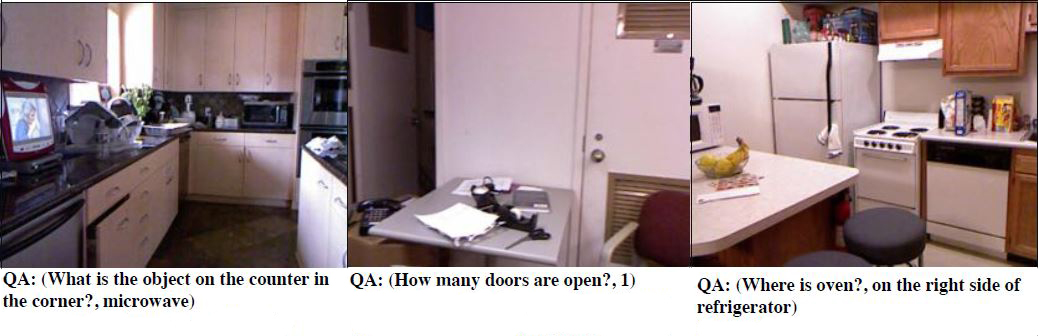
\includegraphics[scale=0.5]{images/DAQUAR.jpg}}
  	\caption[چند نمونه از مجموعه‌داده \lr{DAQUAR}]{چند نمونه از مجموعه‌داده \lr{DAQUAR} \cite{malinowski2014multi}}
  	\label{fig:DAQUARExample}
  \end{figure}

\subsection[مجموعه داده \lr{VQA}]{مجموعه داده \lr{VQA} \cite{antol2015vqa} \cite{goyal2017making}}

مجموعه‌داده
 \lr{Visual Question Answering v1(VQA v1)}
 \footnote{\href{https://visualqa.org/}{https://visualqa.org/}}
یکی از پرکاربردترین مجموعه‌داده‌ها در زمینه پرسش و پاسخ تصویری است. این مجموعه‌داده شامل دو بخش است. یک بخش از تصاویر واقعی ساخته‌شده‌است که
 \lr{VQA-real} 
 نام‌دارد و بخش دیگر با تصاویر کارتونی ساخته‌شده‌است که با نام 
 \lr{VQA-abstract}
 از آن در مقالات یاد می‌شود.
 
 \lr{VQA-real} 
 به ترتیب شامل 123287 تصویر آموزشی و 81434 تصویر آزمایشی است که این تصاویر از مجموعه‌داده
 \lr{MS-COCO}
 \cite{lin2014microsoft}
  تهیه شده است.  برای جمع‌آوری پرسش و پاسخ از نیروی انسانی استفاده‌شده‌است. برای هر تصویر حداقل 3 سوال منحصربه‌فرد وجود دارد و برای هر سوال 10 پاسخ توسط کاربرهای منحصر به فرد جمع‌آوری‌شده‌است. این مجموعه‌داده شامل 614163 سوال به صورت 
  \lr{open-ended}
  و چندگزینه‌ای است. در 
  \cite{antol2015vqa}
  بررسی دقیقی در مورد نوع سوالات، طول سوالات و پاسخ‌ها و غیره انجام‌شده‌است.
  
  
 \lr{VQA-abstract}
 به عنوان یک مجموعه‌داده جداگانه و مکمل در کنار
 \lr{VQA-real}
 قرار دارد. هدف از این مجموعه‌داده از بین بردن نیاز به تجزیه و تحلیل تصاویر واقعی است تا مدل‌ها برای پاسخ به سوالات تمرکز خود را بر روی استدلال‌های سطح بالاتری بگذارند. تصاویر کارتونی در این مجموعه‌داده به صورت دستی توسط انسان‌ها و به وسیله‌ی رابط کاربری که از قبل آماده‌شده‌است؛ ساخته‌شده‌است. تصاویر می‌تواند دو حالت را نشان‌دهند: داخل خانه و خارج از خانه که هر کدام مجموعه متفاوتی از عناصر را شامل می‌شوند از جمله حیوانات، اشیا و انسان‌ها با حالت‌های مختلف. در مجموع 50000 تصویر ایجاد‌شده‌است. مشابه 
 \lr{VQA-real}
 ، 3 سوال برای هر تصویر (یعنی در کل 150000 سوال) و برای هر سوال 10 پاسخ  جمع‌آوری‌شده‌است.
 
 مجموعه‌داده 
\lr{Visual Question Answering v2(VQA v2)}
در سال 2017 پس از مجموعه‌داده 
\lr{VQA v1}
معرفی شد. 
\lr{VQA v2}
نسبت به 
\lr{VQA v1}
متوازن تر است و تعصبات زبانی در 
\lr{VQA v1}
را کاهش داده است. اندازه‌ی مجموعه داده‌ی
\lr{VQA v2}
تقریبا دو برابر مجموعه‌داده‌ی 
\lr{VQA v1}
است. در مجموعه‌داده‌ی
\lr{VQA v2}
تقریبا برای هر سوال دو تصویر مشابه وجود دارد که پاسخ‌های متفاوتی برای سوال دارند.

  \begin{figure}[h]
	\centerline{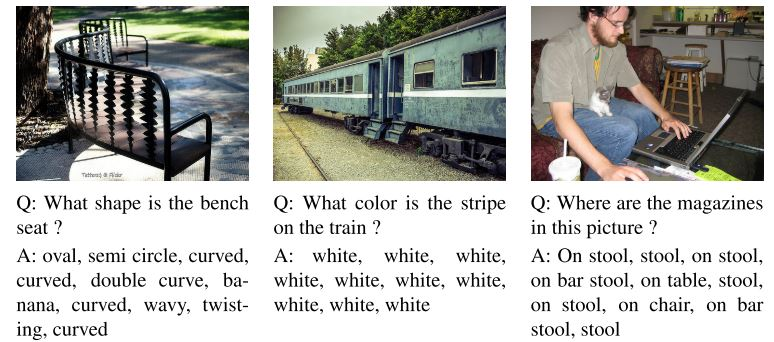
\includegraphics[scale=0.5]{images/VQA1-real.JPG}}
	\caption[چند نمونه از مجموعه‌داده \lr{VQA v1 - real} ]{چند نمونه از مجموعه‌داده \lr{VQA v1 - real} \cite{antol2015vqa}}
	\label{fig:vqa1realExample}
  \end{figure}

  \begin{figure}[h]
	\centerline{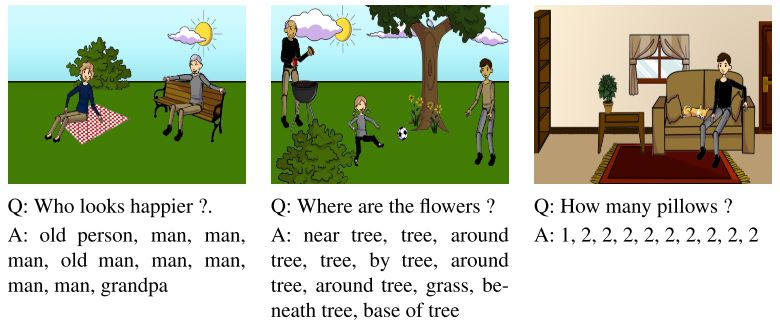
\includegraphics[scale=0.5]{images/VQA1-abstract.JPG}}
	\caption[چند نمونه از مجموعه‌داده \lr{VQA v1 - abstarct}]{چند نمونه از مجموعه‌داده \lr{VQA v1 - abstarct} \cite{antol2015vqa}}
	\label{fig:vqa1abstractExample}
  \end{figure}

  \begin{figure}[h]
	\centerline{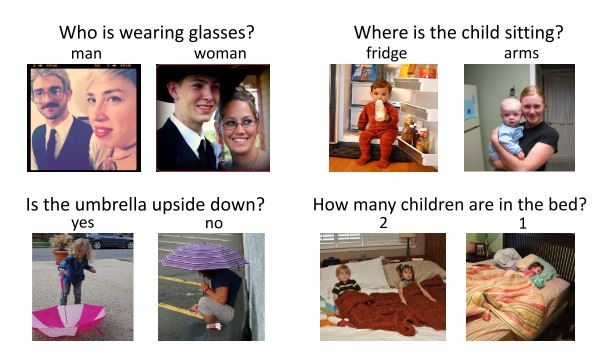
\includegraphics[scale=0.6]{images/VQA2.JPG}}
	\caption[چند نمونه از مجموعه‌داده \lr{VQA v2}]{چند نمونه از مجموعه‌داده \lr{VQA v2} \cite{goyal2017making}}
	\label{fig:vqa2Example}
  \end{figure}

\subsection[مجموعه داده \lr{Visual Madlibs}]{مجموعه داده \lr{Visual Madlibs} \cite{yu2015visual}}

	مجموعه‌داده 
	\lr{Visual Madlibs}
	شکل متفاوتی از پرسش و پاسخ را ارائه می‌دهد. برای هر تصویر جملاتی در نظرگرفته شده‌است و یک کلمه از آن که معمولا مربوط به آدم، اشیا و  فعالیت‌های نمایش‌داده‌شده در تصویر است؛ از جمله حذف‌شده و به جای آن جای‌خالی قرار‌گرفته‌است. پاسخ‌ها کلماتی هستند که این جملات را تکمیل می‌کنند. برای مثال جمله "دو[جای‌خالی]در پارک [جای‌خالی] بازی‌می‌کنند."در وصف یک تصویر بیان‌شده‌است که با دو کلمه "مرد" و "فریزبی" می‌توان جاهای‌خالی‌ را پرکرد. این مجموعه‌داده شامل 10738 تصویر از مجموعه‌داده 
	\lr{MS-COCO}
	\cite{lin2014microsoft}
	 و 360001 جمله با جای‌خالی است. جملات با جای‌خالی به طور خودکار و با استفاده از الگوهای از پیش‌تعیین‌شده تولیدشده‌اند. پاسخ‌ها در این مجموعه‌داده به هر دو شکل 
	\lr{open-ended}
	و چند‌گزینه‌ای است.
  \begin{figure}[h]
	\centerline{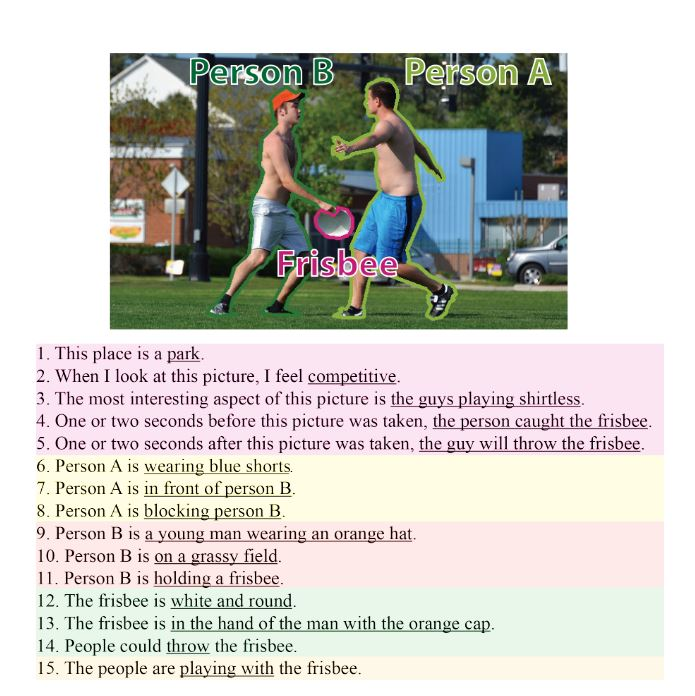
\includegraphics[scale=0.5]{images/visualmadlibs.JPG}}
	\caption[یک نمونه از مجموعه‌داده \lr{Visual Madlibs}]{یک نمونه از مجموعه‌داده \lr{Visual Madlibs} \cite{yu2015visual}}
	\label{fig:visualmadlibsExample}
  \end{figure}

\subsection[مجموعه داده \lr{Visual7w}]{مجموعه داده \lr{Visual7w}\cite{zhu2016visual7w}}
	مجموعه‌داده
 \lr{Visual7W}
	نیز بر اساس مجموعه‌داده
 \lr{MS-COCO}
 \cite{lin2014microsoft}
	  ساخته‌شده‌است. این مجموعه‌داده شامل 47300 تصویر و 327939 جفت سوال و پاسخ است. این مجموعه‌داده همچنین از 1311756 پرسش و پاسخ چند‌گزینه‌ای تشکیل‌شده‌است که هر سوال 4 گزینه دارد و تنها یکی از گزینه‌ها پاسخ صحیح سوال است. برای جمع‌آوری سوالات چندگزینه‌ای توسط انسان‌ها از پلتفرم آنلاین 
  \lr{Amazon Mechanical Turk}
  استفاده‌شده‌است. نکته‌ی حائز اهمیت در این ‌مجموعه‌داده این است که تمامی اشیایی که در متن پرسش یا پاسخ ذکر‌شده‌است، به نحوی به کادر محدود‌کننده‌ی آن شی در تصویر مرتبط شده‌است. مزیت این روش، رفع ابهام‌های موجود در متن است.  همان‌طور که از نام این مجموعه‌داده پیداست؛ سوالات آن با 7 کلمه‌ی پرسشی که حرف اول آن w است شروع می‌شود. این 7 کلمه شامل
  \lr{what}
  ،
  \lr{where}
  ،
  \lr{when}
  ،
  \lr{who}
  ،
  \lr{why}
  ،
  \lr{how}
  و
  \lr{which}
	است. پرسش‌های
  \lr{Visual7W}
	 نسبت به به مجموعه‌داده 
  \lr{VQA v1}
  غنی‌تر و سخت‌تر است. همچنین پاسخ‌ها طولانی‌تر هستند.
  \begin{figure}[h]
  	\centerline{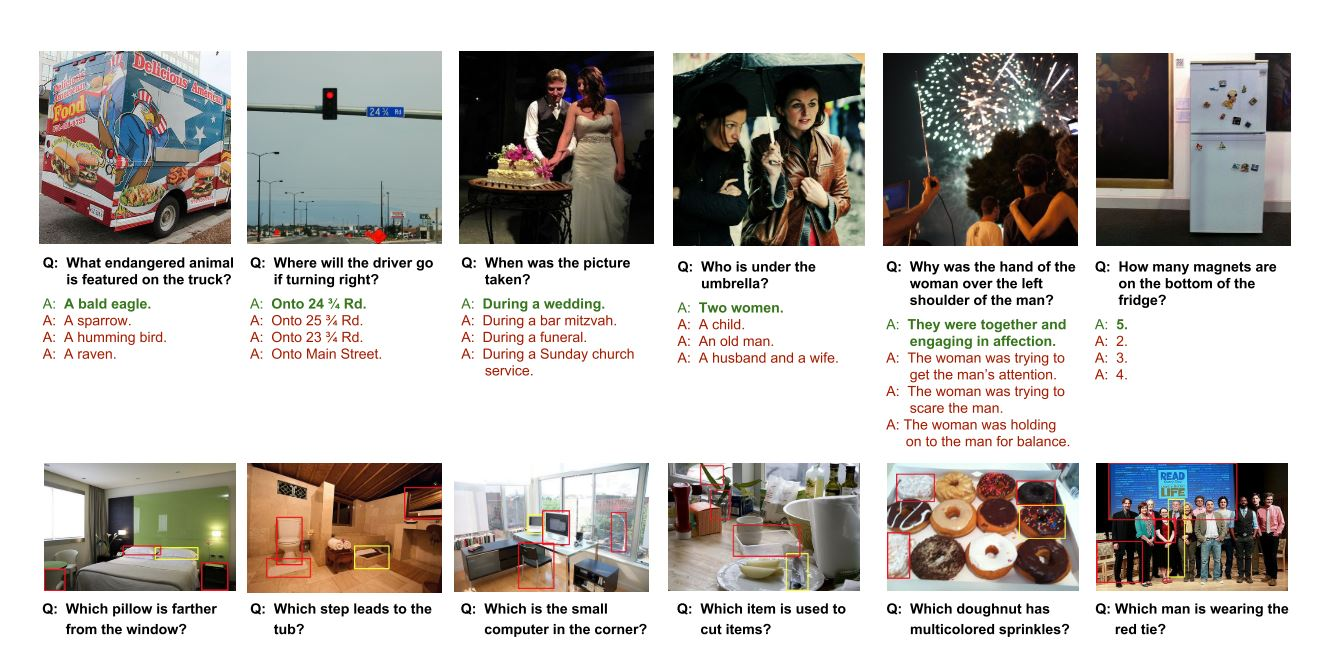
\includegraphics[scale=0.5]{images/Visual7W.JPG}}
  	\caption[چند نمونه از مجموعه‌داده \lr{Visual7W}]{چند نمونه از مجموعه‌داده
  		 \lr{Visual7W} \cite{zhu2016visual7w}. 
  		 ردیف اول،پاسخ‌های سبز رنگ، پاسخ صحیح هستند و پاسخ‌های قرمز پاسخ‌های نادرست تولید شده توسط انسان است. ردیف دوم، کادر زرد جواب صحیح است و کادرهای قرمز پاسخ‌های اشتباه انسانی است.}
  	\label{fig:Visual7WExample}
  \end{figure}
  
\subsection[مجموعه داده \lr{CLEVR}]{مجموعه داده \lr{CLEVR}\cite{johnson2017clevr}}

\lr{CLEVR}
 یک مجموعه‌داده برای ارزیابی درک بصری سیستم‌های 
 \lr{VQA}
  است. تصاویر این مجموعه‌داده با استفاده از سه شی استوانه، کره و مکعب تولیدشده‌است. برای هر کدام از این اشیا دو اندازه متفاوت، دو جنس متفاوت و هشت رنگ مختف در نظر گرفته شده است. سوالات هم به طور مصنوعی بر اساس مکانی که اشیا در تصوبر قرار گرفته اند؛ ایجاد شده‌است. سوالات در
   \lr{CLEVR }
   به گونه‌ای طراحی‌شده‌است که جنبه‌های مختلف استدلال بصری توسط سیستم‌های 
   \lr{VQA}
   را مورد ارزیابی قرار می‌دهد از جمله شناسایی ویژگی، شمارش اشیا، مقایسه، روابط مکانی اشیا و عملیات منطقی. در این مجموعه‌داده مکان تصاویر نیز با استفاده از یک مستطیل مشخص‌شده‌است.
   
   \begin{figure}[h]
   	\centerline{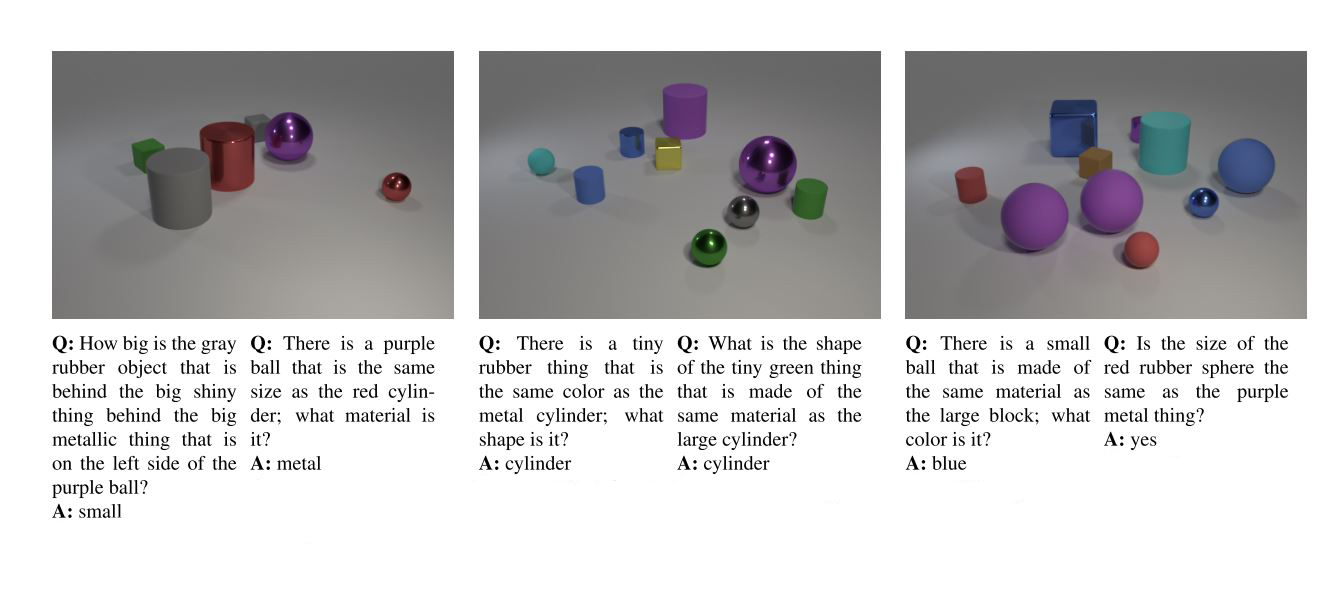
\includegraphics[scale=0.4]{images/CLEVR.JPG}}
   	\caption[چند نمونه از مجموعه‌داده\lr{CLEVR}]{چند نمونه از مجموعه‌داده\lr{CLEVR} \cite{johnson2017clevr}.}
   	\label{fig:CLEVRExample}
   \end{figure}

\subsection[مجموعه داده \lr{Tally-QA}]{مجموعه داده \lr{Tally-QA}\cite{acharya2019tallyqa}}

	در سال 2019، مجموعه‌داده 
   \lr{Tally-QA}
منتشر شد که بزرگ‌ترین مجموعه‌داده پرسش و پاسخ تصویری برای شمارش اشیا است. اکثر مجموعه‌داده‌های شمارش اشیا در پرسش و پاسخ تصویری دارای سوالات ساده هستند که برای پاسخ‌دادن به این سوال‌‌ها تنها کافی است که اشیا در تصویر تشخیص‌داده‌شوند. بنابراین، این موضوع باعث ایجاد مجموعه‌داده‌ی 
   \lr{Tally-QA}
  شد که علاوه بر سوالات ساده، سوالات پیچیده را نیز در بر می‌گیرد که برای پاسخ دادن به آن‌ها به استدلال بیشتری از تشخیص اشیا نیاز است. تعداد سوالات ساده در
  \lr{Tally-QA} 
  برابر با 211430 و تعداد سوالات پیچیده برابر با 76477 است. سوالات ساده این مجموعه‌داده از مجموعه‌داده‌های دیگری( 
  \lr{VQA v2} \cite{goyal2017making}
  و 
  \lr{Visual Genome} \cite{krishna2017visual}
  ) برداشته‌شده‌است و سوالات پیچیده با استفاده از 800 کاربر انسانی از طریق پلتفرم آنلاین 
 \lr{Amazon Mechanical Turk}
  جمع‌آوری شده‌است. مجموعه‌داده 
  \lr{Tally-QA} 
  به سه بخش آموزش و تست-ساده و تست-پیچیده تقسیم می‌شود. بخش تست-ساده تنها شامل سوالات ساده و بخش تست-پیچیده تنها دارای سوالات پیچیده‌ای است که از 
  \lr{Amazon Mechanical Turk}
  جمع‌آوری شده‌است. 

   \begin{figure}[h]
		\centerline{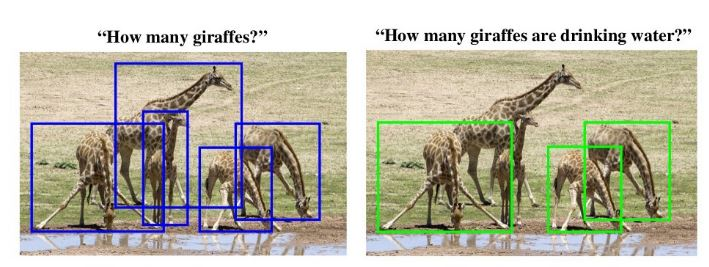
\includegraphics[scale=0.8]{images/TallyQA.JPG}}
		\caption[چند نمونه از مجموعه‌داده\lr{Tally-QA}]{چند نمونه از مجموعه‌داده\lr{Tally-QA} \cite{acharya2019tallyqa}.عکس سمت چپ یک نمونه از سوالات ساده و عکس سمت راست یک نمونه از سوالات پیچیده است.}
		\label{fig:TallyQAExample}
	\end{figure}

\subsection[مجموعه داده \lr{KVQA}]{مجموعه داده \lr{KVQA}\cite{shah2019kvqa}}
	مجموعه داده 
	\lr{KVQA}
	 که مخفف
	\lr{Knowledge-based Visual Question Answering}
	است در سال 2019 طراحی شده است به طوری که بر خلاف مجموعه‌داده‌های قبلی، برای پیدا کردن پاسخ سوالات نیاز به دانش خارجی دارد. بدین منظور این مجموعه داده شامل 183هزار پرسش و پاسخ در مورد 18هزار شخص معروف شامل ورزشکاران، سیاستمداران و هنرمندان است.  اطلاعات و تصاویر مرتبط با این  اشخاص از
	\lr{Wikidata}
	و
	\lr{Wikipedia}
	استخراج شده است.
	\lr{KVQA}
شامل 24هزار تصویر است. این مجموعه‌داده به صورت تصادفی به سه بخش آموزش، ارزیابی و آزمون به ترتیب با نسبت های
	\lr{0.7}
 	، 
 	\lr{0.2}
  و
  	\lr{0.1}
   تقسیم شده است. تنوع پرسش و پاسخ ها در 
	\lr{KVQA}
	به گونه‌ای در نظر گرفته شده است که مشکل همیشگی بایاس در مجموعه‌داده‌های پرسش و پاسخ تصویری، در این مجموعه داده وجود نداشته باشد.
   \begin{figure}[h]
		\centerline{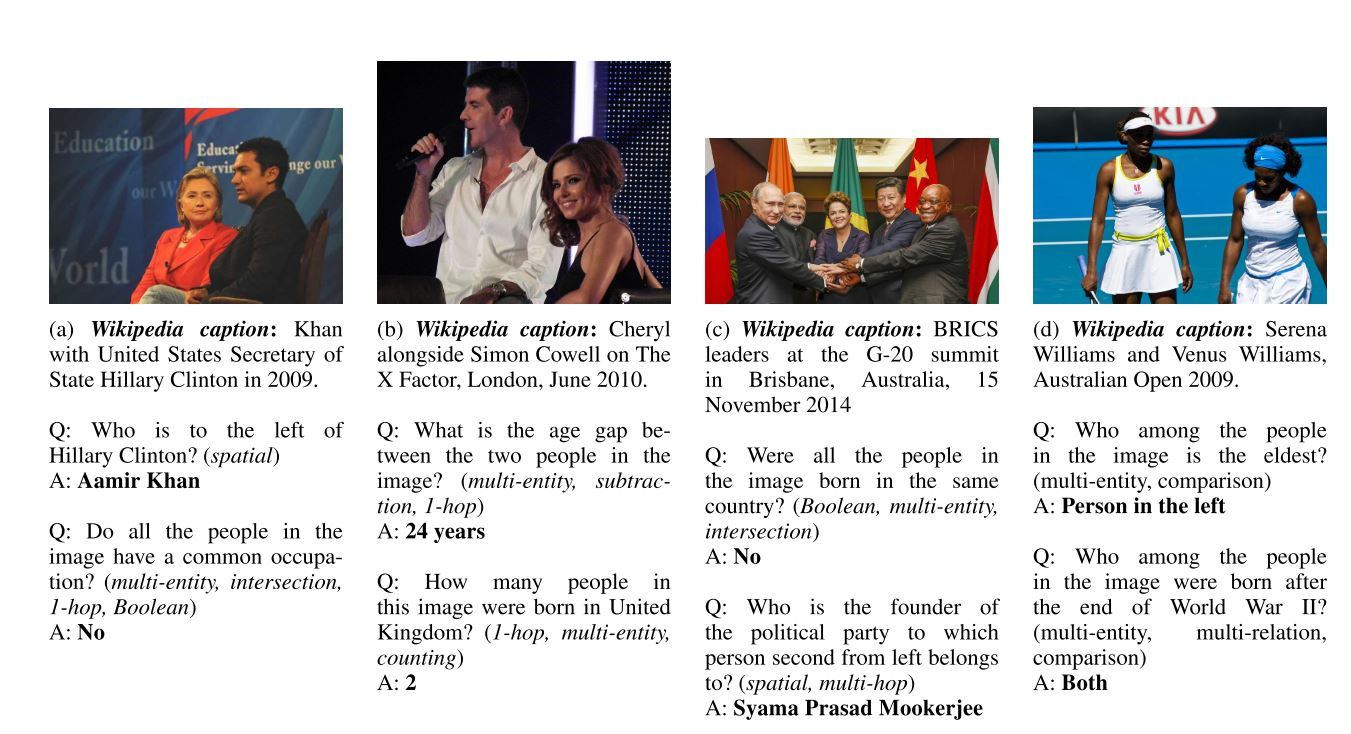
\includegraphics[scale=0.4]{images/KVQA.JPG}}
		\caption[چند نمونه از مجموعه‌داده\lr{KVQA}]{چند نمونه از مجموعه‌داده\lr{KVQA} \cite{shah2019kvqa}}.
		\label{fig:KVQAExample}
    \end{figure}

\section{تقویت مجموعه‌داده در مسئله پرسش و پاسخ تصویری}
به لطف توسعه سریع شبکه‌های عصبی عمیق مسئله پرسش و پاسخ تصویری به موفقیت‌های بزرگی دست یافته است. مطالعات نشان می‌دهد که عملکرد شبکه‌های عصبی عمیق به میزان داده‌های آموزشی بستگی دارد و همیشه از داده‌های آموزشی بیشتر سود می‌برند. یکی از ترفندهای اصلی در شبکه‌های عصبی عمیق تقویت داده
\footnote{\lr{data augmentation}}
 است که به طور گسترده در بسیاری از مسائل پردازش تصویر و بینایی ماشین مورد استفاده قرار می‌گیرد. اما مقالات کمی وجود دارد که مسئله تقویت داده را در پرسش و پاسخ تصویری بررسی کرده‌اند. یکی از چالش‌های تقویت داده در مسئله پرسش و پاسخ تصویری این است که هیچ یک از روش‌های تقویت داده مبتنی بر تصویر مانند چرخش
 \footnote{rotation}
 و ورق زدن
 \footnote{flipping}
  نمی‌توانند مستقیماً بر روی مسئله پرسش و پاسخ تصویری اعمال شود زیرا ساختار معنایی آن حفظ نخواهد شد. به عنوان مثال با چرخش یک تصویر ممکن است پرسش و پاسخ مرتبط با آن( مانند «ماشین در سمت چپ یا راست سطل زباله است؟») دیگر درست نباشد.
  
  در
  \cite{kafle2017data}
 برای اولین بار دو روش برای تقویت داده در مسئله پرسش و پاسخ تصویری پیشنهاد شد.  در روش اول برای تولید پرسش و پاسخ از الگو استفاده‌ می‌شود. برای تولید الگو از حاشیه‌نویسی 
 \footnote{annotation}
 موجود در مجموعه‌داده استفاده‌ می‌شود. با استفاده از این روش 4 نوع سوال تولید می‌شود: (1) سوالات بله و خیر (2) سوالات شمارشی (3) تشخیص شی، صحنه و یا فعالیت (4) تشخیص ورزش. برای مثال برای تولید سوالات بله و خیر، با استفاده از حاشیه‌نویسی موجود در مجموعه ‌داده لیستی از اشیا موجود در تصویر آماده می‌شود. سپس اگر محدوده مربوط به اشیا بزرگتر از 2000 پیکسل باشد، سوالی مانند « آیا [شی] در تصویر وجود دارد؟» تولید می‌شود که پاسخ آن هم «بله» است. به همین ترتیب با استفاده از دانشی که از مجموعه‌داده می‌توان بدست آورد؛ برای سایر انواع سوالات الگویی برای تولید سوال و پاسخ آن تولید می‌شود. یکی از مشکلات این روش برای تقویت داده این است که سوالات تولید شده انعطاف‌‌پذیر نیستند و ممکن است شباهت زیادی به نحوه‌ی طرح سوالات موجود در مجموعه‌داده نداشته باشند. به همین علت، روش دیگری در 
 \cite{kafle2017data}
 مبتنی بر 
 \lr{LSTM}
 برای تولید سوال برای هر تصویر پیشنهاد شده است. این شبکه از دو لایه 
 \lr{LSTM}
 تشکیل شده است که هر کدام دارای 1000 واحد مخفی است و پس از آن‌ها نیز دو لایه‌ی کاملا متصل که هر کدام 7000 نورون مخفی دارند(برابر با تعداد واژگان) ساخته شده است. برای تولید سوال، در ابتدا توکن شروع سوال به همراه ویژگی‌های تصویر به شبکه داده‌ می‌شود. برای هر تصویر 30 سوال تولید می‌شود که تنها سه تا از پرتکرارترین سوالات  نگه داشته می‌شود. برای پیدا کردن جواب سوال‌های تولیده شده توسط شبکه 
 \lr{LSTM}
 از یک شبکه‌ی ساده
 \lr{MLP}
 که در 
 \cite{kafle2016answer}
  پیشنهاد شده است؛ استفاده شده است. در 
 \cite{kafle2017data}
  نشان دادند که استفاده از این دو روش برای تقوبت داده‌ها منجر به بهبود عملکرد روش‌های موجود برای حل مسئله پرسش و پاسخ تصویری می‌شود. 
  
  اخیرا در
 \cite{tang2020semantic}
 برای تقویت داده روشی مبتنی بر تولید نمونه‌های خصمانه
 \footnote{\lr{adversarial examples}}
 پیشنهاد شده است که بر خلاف کارهای قبلی، تقویت داده هم برای تصاویر و هم برای سوالات انجام می‌شود.
 
 
\section{بررسی فازهای مختلف مسئله پرسش و پاسخ تصویری}
بسیاری از محققان راه‌حل‌ها یا الگوریتم‌هایی را برای حل مسئله پرسش و پاسخ تصویری پیشنهاد‌کرده‌اند که به طور کلی می‌توان آن را به یک فرآیند سه فازی تقسیم‌بندی کرد. فاز اول این فرآیند استخراج ویژگی از تصویر و سوالات است که راه‌حل‌های موفق در این فاز ریشه در روزهای باشکوه یادگیری عمیق دارد زیرا بیشتر راه‌حل‌های موفق در این حوزه از مدل‌های یادگیری عمیق استفاده می‌کنند مانند 
  \lr{CNN}
 ها برای استخراج ویژگی از  تصویر و 
  \lr{RNN}
  ها و انواع آن(
  \lr{LSTM}
  و
  \lr{GRU}
  ) برای استخراج ویژگی از سوالات. در فاز دوم که مهم‌ترین و اصلی‌ترین فاز می‌باشد، ویژگی‌های استخراج شده از تصویر و سوال باهم ترکیب می‌شوند. سپس از ترکیب ویژگی‌ها برای تولید پاسخ نهایی در فاز سوم استفاده می‌شود.
\subsection{فاز 1 : استخراج ویژگی از تصویر و سوا ل} \label{sec:extract}

		استخراج ویژگی از تصویر و سوال مرحله‌ی مقدماتی در پرسش و پاسخ تصویری است. ویژگی تصویر، تصویر را به عنوان یک بردار عددی  توصیف می‌کند تا بتوان به راحتی عملیات‌های مختلف ریاضی را بر روی آن اعمال کرد. روش‌های زیادی وجود دارد که به صورت مستقیم از تصویر ویژگی استخراج می‌کنند مانند بردار ساده 
		\lr{RGB}
		،
		\lr{SIFT}
		، تبدیل
		\lr{HAAR}
		و 
		\lr{HOG}.
		اما با ظهور شبکه‌های یادگیری عمیق، نیاز به استخراج ویژگی به صورت مستقیم از بین رفت زیرا این شبکه‌ها قادر به یادگیری ویژگی هستند. آموزش مدل‌های یادگیری عمیق به منابع محاسباتی گران قمیت و مجموعه‌داده‌های بزرگ نیاز دارد. از این رو، استفاده از مدل‌های شبکه عصبی عمیق از قبل آموزش دیده، استخراج ویژگی‌ از تصاویر را به راحتی امکان‌پذیر می‌کنند. 
		
		یکی از بهترین شبکه‌های عصبی برای استخراج ویژگی از تصویر، شبکه‌های عصبی کانولوشنی هستند. 
		\begin{table}
			\caption{بررسی اجمالی مهم‌ترین شبکه‌های عصبی کانولوشنی که بر روی مجموعه‌داده
				\lr{ImageNet}
				آموزش ‌داده شده‌اند.}
			\label{tabel:2}
			\begin{center}
				\begin{tabular}{ |c|c|c|c|c| } 
					\hline
					\textbf{مدل \lr{CNN}} & \textbf{سال} & \textbf{تعداد لایه‌‌ها} & \textbf{ابعاد ورودی}  & \textbf{ابعاد خروجی(تعداد ویژگی‌ها)} \\
					\hline \hline
					\textbf{\lr{AlexNet}\cite{hinton2012imagenet}} & 2012 & 8 & 227×227 & 4096 \\
					\hline
					\textbf{\lr{VGGNet}\cite{simonyan2014very}} & 2014 & 19 & 224×224 & 4096 \\
					\hline
					\textbf{\lr{GoogleNet}\cite{szegedy2015going}} & 2014 & 22 & 229×229 & 1024 \\
					\hline
					\textbf{\lr{ResNet}\cite{he2016deep}} & 2015 & 152 & 224×224 & 20148\\
					\hline
				\end{tabular}
			\end{center}
		\end{table}
		 در جدول 
		\ref{tabel:2}
		چند نمونه از برجسته‌ترین شبکه‌های عصبی کانولوشنی که بر روی مجموعه‌داده
		\lr{ImageNet}
		\cite{deng2009imagenet}
		آموزش ‌داده شده‌اند؛
		آورده شده است. بیشتر مدل‌های ارائه‌شده در پرسش و پاسخ تصویری از این شبکه‌های عصبی کانولوشنی استفاده می‌کنند تا محتوای تصویری خود را به بردار‌هایی عددی تبدیل کنند.
		\begin{table}
			\caption{شبکه‌های عصبی کانولوشنی استفاده شده در مدل‌های پرسش و پاسخ تصویری.}
			\label{tabel:3}
			\begin{center}
				\begin{tabular}{ |c|c|c|c|c| } 
					\hline
					\textbf{مدل پرسش و پاسخ تصویری} & \textbf{AlexNet} & \textbf{VGGNet} & \textbf{GoogleNet}  & \textbf{ResNet}\\
					\hline \hline
					\textbf{\lr{Image\_QA}\cite{ren2015image}} &  & \checkmark&  & \\
					\hline
					\textbf{\lr{Talk\_to\_Machine}\cite{gao2015you}} &  &  & \checkmark &  \\
					\hline
					\textbf{\lr{VQA}\cite{antol2015vqa}} &  & \checkmark &  &  \\
					\hline
					\textbf{\lr{Vis\_Madlibs}\cite{yu2015visual}} & \checkmark &  &  & \\
					\hline
					\textbf{\lr{VIS + LSTM}\cite{ren2015exploring}} &  & \checkmark  &  & \\
					\hline
					\textbf{\lr{Ahab}\cite{wang2015explicit}} &  & \checkmark &  &  \\
					\hline
					\textbf{\lr{ABC-CNN}\cite{chen2015abc}} &  & \checkmark &  & \\
					\hline
					\textbf{\lr{Comp\_QA}\cite{andreas2015deep}} &  & \checkmark &  & \\
					\hline
					\textbf{\lr{DPPNet}\cite{noh2016image}} &  & \checkmark &  & \\
					\hline
					\textbf{\lr{Answer\_CNN}\cite{Ma2016LearningTA}} &  & \checkmark &  & \\
					\hline
					\textbf{\lr{VQA-Caption}\cite{lin2016leveraging}} &  & \checkmark &  & \\
					\hline
					\textbf{\lr{Re\_Baseline}\cite{jabri2016revisiting}} &  &  &  & \checkmark\\
					\hline
					\textbf{\lr{MCB}\cite{fukui2016multimodal}} &  &  &  & \checkmark \\
					\hline
					\textbf{\lr{SMem-VQA}\cite{xu2016ask}} &  &  & \checkmark & \\
					\hline
					\textbf{\lr{Region\_VQA}\cite{shih2016look}} &  & \checkmark &  & \\
					\hline
					\textbf{\lr{Vis7W}\cite{zhu2016visual7w}} &  & \checkmark &  & \\
					\hline
					\textbf{\lr{Ask\_Neuron}\cite{malinowski2017ask}} & \checkmark & \checkmark & \checkmark & \checkmark \\
					\hline
					\textbf{\lr{SCMC}\cite{cao2017jointly}} &  &  &  & \checkmark \\
					\hline
					\textbf{\lr{HAN}\cite{malinowski2018learning}} &  &  &  & \checkmark\\
					\hline
					\textbf{\lr{StrSem}\cite{yu2018beyond}} &  & \checkmark &  & \\
					\hline
					\textbf{\lr{AVQAN}\cite{ruwa2018affective}} &  &  &  & \checkmark \\
					\hline
					\textbf{\lr{CMF}\cite{lao2018cross}} &  &  &  & \checkmark\\
					\hline
					\textbf{\lr{EnsAtt}\cite{lioutas2018explicit}} &  &  &  & \checkmark \\
					\hline
					\textbf{\lr{MetaVQA}\cite{teney2018visual}} &  &  &  & \checkmark\\
					\hline
					\textbf{\lr{DA-NTN}\cite{bai2018deep}} &  &  &  & \checkmark \\
					\hline
					\textbf{\lr{QGHC}\cite{cao2017jointly}} &  &  &  & \checkmark\\
					\hline
					\textbf{\lr{QTA}\cite{shi2018question}} &  &  &  & \checkmark\\
					\hline
					\textbf{\lr{WRAN}\cite{peng2019word}} &  &  &  & \checkmark \\
					\hline
					\textbf{\lr{QAR} \cite{toor2019question}} &  &  &  & \checkmark \\
					\hline
				\end{tabular}
			\end{center}
		\end{table}
		جدول 
		\ref{tabel:3}
		لیستی از مدل‌های استفاده شده برای حل مسئله پرسش و پاسخ تصویری را نشان می‌دهد و مشخص می‌کند که هر کدام از این مدل‌ها برای استخراج ویژگی از تصویر از کدام یک از شبکه‌های عصبی کانولوشنی موجود در جدول 
		\ref{tabel:2}
		بهره می‌برد. همان‌طور که واضح است 
		\lr{VGGNet}
		و
		\lr{ResNet}
		به طور گسترده‌ای در سیستم‌های پرسش و پاسخ تصویری مورد استفاده قرار گرفته‌اند. یکی از دلایلی که محققان
		\lr{VGGNet}
		 را ترجیح می‌دهند این است که ویژگی‌هایی را استخراج می‌کند که عمومیت بیشتری دارد و برای مجموعه‌داده‌هایی غیر از
		\lr{ImageNet }
		که این مدل‌ها بر روی آن‌ها آموزش داده می‌شوند، موثرتر هستند. دلایل دیگر شامل همگرایی سریع در
		\lr{fine-tuning}
		و پیاده‌سازی ساده در مقایسه با
		\lr{GoogLeNet} 
		و
		\lr{ResNet}
		است. نکته‌ی قابل توجه دیگر در جدول 
		\ref{tabel:3}
		روند مهاجرت از 
		\lr{VGGNet}
		به
		\lr{ResNet}
		در مقالات اخیر است. زیرا در سال‌های اخیر، منابع محاسباتی کافی با هزینه مناسب در دسترس محققان می‌باشد.
		
		بیشتر الگوریتم‌های یادگیری ماشین و یادگیری عمیق  قادر به پردازش متن به شکل خام وساده نیستند  و برای بازنمایی متن‌ها نیاز به 
		\lr{word embedding}
		دارند. مسئله پرسش و پاسخ تصویری نیز از این قاعده مستثنا نیست و باید برای بازنمایی سوالات از 
		\lr{word embedding}
		استفاده کند.
	 \lr{word embedding}
	 نگاشت کلمات یا عبارات از واژگان به بردارهای عددی است تا کامپیوترها بتوانند به راحتی آن‌ها را پردازش کنند. 
	 \lr{word embedding}
	 عمدتاً برای مدل‌سازی زبان و یادگیری ویژگی در پردازش زبان طبیعی استفاده می‌شود. ایده اصلی در پشت تمام روش‌های
	 \lr{word embedding}
	 ، گرفتن هرچه بیشتر اطلاعات معنایی و ریخت‌شناسی است. 
	 
	 روش‌های 
	 \lr{word embedding}
	 بسیاری در مسئله پرسش و پاسخ تصویری استفاده شده است. در ادامه به برجسته‌ترین و پرکاربردترین روش‌های
	 \lr{word embedding}
	  موجود و استفاده‌شده در مسئله پرسش و پاسخ تصویری می‌پردازیم و معایب و مزایای هر کدام را بررسی خواهیم کرد.
	  
	  روش کدگذاری
	  \lr{one-hot}
	  ساده‌ترین روش
	  \lr{word embedding}
	  است. در این روش یک لغت‌‌نامه از همه واژه‌های منحصربه‌فرد موجود در مجموعه‌داده ساخته‌می‌شود و اندیس یکتایی به هر واژه اختصاص می‌یابد. بنابراین برای هر واژه یک بردار به طول تعداد واژ‌ه‌ها ساخته می‌شود که تمامی مقادیر آن صفر است به جز اندیس مربوط به همان واژه که مقدار آن یک است. پیاده‌سازی این روش آسان است اما طول بردارها  بزرگ است زیرا برابر با تعداد کل واژه‌های منحصر به فرد مجموعه داده است و هزینه زیادی برای ذخیره‌سازی دارد. بزرگترین عیب این روش  این است که نمی‌توان از آن معنا  و مفهوم استخراج کرد زیرا فاصله‌ی تمامی کلمات با هم یکسان است. در صورتی که ما انتظار داریم؛ کلماتی که مشابه هم هستند بردارهای نزدیک به هم یا مشابه هم داشته باشند و کلملاتی که معنای متفاوتی با یکدیگر دارند تا حد امکان بردارهایشان از هم دور باشند.  
		
		برای رفع مشکلات کدگذاری 
		\lr{one-hot}
		 ، دو روش
		\lr{CBOW} 
		\footnote{\lr{Continouse Bag Of Words}}
		\cite{mikolov2013efficient}
		 و
		\lr{Skip-gram}
		\cite{mikolov2013efficient}
		پیشنهاد شد که از شبکه‌های عصبی به عنوان جز اصلی خود استفاده می‌کنند. این دو مدل بر عکس هم کار می‌کنند.	در هر دو مدل، از یک شبکه عصبی سه لایه که شامل لایه ورودی، لایه پنهان ولایه خروجی است، استفاده شده است. درمدل 
		\lr{CBOW} 
		 کلمات اطراف و نزدیک به یک کلمه(
		 \lr{n-1}
		 کلمه) به لایه ورودی داده می‌شود و مدل سعی می‌کند این کلمه(n امین کلمه) را حدس بزند.  بعد از آموزش این شبکه‌، وزن بین لایه‌ی پنهان و لایه خروجی کلمات مجموعه داده را بازنمایی می‌کند که هر ستون آن بردار مربوط به یک کلمه را نشان می‌دهد. در مدل
		\lr{skip-gram}
		برعکس 
		\lr{CBOW} 
		یک کلمه به شبکه ورودی داده می‌شود و شبکه باید کلمات اطراف و نزدیک به آن را حدس بزند. 
		\begin{figure}
			\centerline{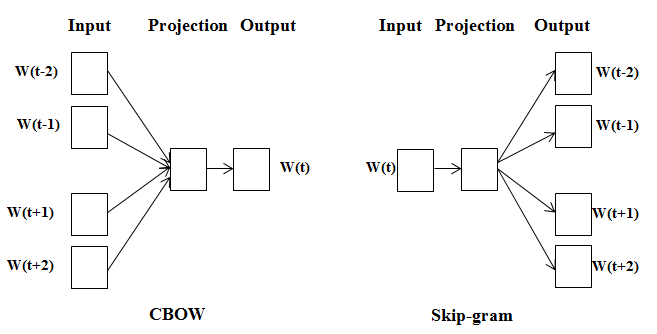
\includegraphics[scale=0.5]{images/2.png}}
			\caption{
		معماری شبکه 
			\lr{CBOW}
			و
			\lr{Skip-gram}	
			}
			\label{fig:CBOW&skip-gram}
		\end{figure}
		معماری 
		\lr{CBOW}
		و
		\lr{Skip-gram}
		در شکل 
		\ref{fig:CBOW&skip-gram}
	آورده شده است.
	
		 یکی دیگر از 
		 \lr{word embedding}
		های مشهور، مدل بردار سراسری یا به اختصار 
		 \lr{GloVe}
		 \footnote{\lr{Global Vector}}
		 است که توسط پنینگتون و همکاران 
		 \cite{pennington2014glove}
		 در سال 2014 در تیم پردازش زبان‌های طبیعی دانشگاه استنفورد معرفی و توسعه داده شد. آیا نیاز به توضیح کامل این روش است؟
		 
		 با پیشرفت یادگیری عمیق در دهه اخیر، محققان برای استخراج ویژگی و بازنمایی متن از
		 \lr{CNN}
		 ،
		 \lr{LSTM‌}
		 \cite{hochreiter1997long}
		  و
		 \lr{GRU}
		 \cite{cho2014learning}
		 استفاده کردند. در مسئله پرسش و پاسخ تصویری برای استخراج ویژگی از سوال با استفاده از 
		 \lr{CNN}
		 بردارهای کلمات سوال در کنار هم قرار داده می‌شود سپس به لایه‌های کانولوشنی یک بعدی داده می‌شود و فیلتر‌های متفاوتی بر روی آن‌ها اعمال می‌شود و پس از عبور از لایه‌ 
		 \lr{max-pooling}
		 ویژگی‌ها بدست می‌آید.
		 
		 توضیح 
		 \lr{LSTM}
		 لازمه؟
		 
		 توضیح 
		 \lr{GRU}
		 لازمه؟
		 
		 مدل‌های مختلف در مسئله پرسش و پاسخ تصویری از 
		 \lr{word embedding}
		 های ذکر شده در بالا برای تولید بردار ویژگی برای سوال‌ها استفاده کرده‌اند.
		 \begin{table}
		 	\caption{
		 		\lr{word embedding}
		 		های استفاده شده در مدل‌های پرسش و پاسخ تصویری.}
		 	\label{tabel:4}
		 	\begin{center}
		 		\resizebox{\textwidth}{!}{\begin{tabular}{ |c|c|c|c|c|c|c|c| } 
		 			\hline
		 			\textbf{مدل پرسش و پاسخ تصویری} & \textbf{\lr{one-hot}} & \textbf{\lr{CBOW}} & \textbf{\lr{Skip-gram/Word2vec}}  & \textbf{\lr{GloVe}} & \textbf{\lr{CNN}} & 
		 			\textbf{\lr{LSTM}} & \textbf{\lr{GRU}}\\
		 			\hline \hline
		 			\textbf{\lr{Image\_QA}\cite{ren2015image}} &  &  & \checkmark &  &  &  & \\
		 			\hline
		 			\textbf{\lr{Talk\_to\_Machine}\cite{gao2015you}} &  &  &  &  &  & \checkmark &    \\
		 			\hline
		 			\textbf{\lr{VQA}\cite{antol2015vqa}} &  & \checkmark &  &  &  &  &  \\
		 			\hline
		 			\textbf{\lr{Vis\_Madlibs}\cite{yu2015visual}} &  &  & \checkmark &  &  &  &  \\
		 			\hline
		 			\textbf{\lr{VIS + LSTM}\cite{ren2015exploring}} &  &  &  &  &  & \checkmark &  \\
		 			\hline
		 			\textbf{\lr{ABC-CNN}\cite{chen2015abc}} &  &  &  &  &  & \checkmark &  \\
		 			\hline
		 			\textbf{\lr{Comp\_QA}\cite{andreas2015deep}} &  &  &  &  &  & \checkmark &  \\
		 			\hline
		 			\textbf{\lr{DPPNet}\cite{noh2016image}} &  &  &  &  &  &  & \checkmark \\
		 			\hline
		 			\textbf{\lr{Answer\_CNN}\cite{Ma2016LearningTA}} &  &  &  &  & \checkmark &  &  \\
		 			\hline
		 			\textbf{\lr{VQA-Caption}\cite{lin2016leveraging}} &  &  &  &  &  & \checkmark &  \\
		 			\hline
		 			\textbf{\lr{Re\_Baseline}\cite{jabri2016revisiting}} &  &  & \checkmark &  &  &  & \\
		 			\hline
		 			\textbf{\lr{MCB}\cite{fukui2016multimodal}} &  &  &  &   &  & \checkmark &  \\
		 			\hline
		 			\textbf{\lr{SMem-VQA}\cite{xu2016ask}} &  & \checkmark &   &  &  &  & \\
		 			\hline
		 			\textbf{\lr{Region\_VQA}\cite{shih2016look}} &  &  & \checkmark &  &  &  &  \\
		 			\hline
		 			\textbf{\lr{Vis7W}\cite{zhu2016visual7w}} & \checkmark &  &  &  &  &  &  \\
		 			\hline
		 			\textbf{\lr{Ask\_Neuron}\cite{malinowski2017ask}} &  & \checkmark &  &  & \checkmark & \checkmark & \checkmark  \\
		 			\hline
		 			\textbf{\lr{SCMC}\cite{cao2017jointly}} &  &  &  &  & \checkmark &  &  \\
		 			\hline
		 			\textbf{\lr{HAN}\cite{malinowski2018learning}} &  &  &  &  &  & \checkmark & \\
		 			\hline
		 			\textbf{\lr{StrSem}\cite{yu2018beyond}} &  &  &  &  &  & \checkmark &  \\
		 			\hline
		 			\textbf{\lr{AVQAN}\cite{ruwa2018affective}} & \checkmark &  &  &  &  &  &  \\
		 			\hline
		 			\textbf{\lr{CMF}\cite{lao2018cross}} &  &  &  & \checkmark  &  & \checkmark & \\
		 			\hline
		 			\textbf{\lr{EnsAtt}\cite{lioutas2018explicit}} &  &  &  & \checkmark  &  &  &  \\
		 			\hline
		 			\textbf{\lr{MetaVQA}\cite{teney2018visual}} &  &  &  & \checkmark  &  &  & \checkmark\\
		 			\hline
		 			\textbf{\lr{DA-NTN}\cite{bai2018deep}} &  &  &  &  &  &  & \checkmark \\
		 			\hline
		 			\textbf{\lr{QGHC}\cite{cao2017jointly}} &  &  &  &  &  &  & \checkmark \\
		 			\hline
		 			\textbf{\lr{WRAN} \cite{peng2019word}} &  &  &  &   &  &  & \checkmark \\
		 			\hline
		 			\textbf{\lr{QAR}\cite{toor2019question}} &  &  &  & \checkmark  &  &  &  \\
		 			\hline
		 		\end{tabular}}
		 	\end{center}
		 \end{table}
		 جدول 
		 \ref{tabel:4}
		 لیستی از مدل‌های پرسش و پاسخ تصویری به همراه 
		 \lr{word embedding}
		 استفاده شده در آن‌ها را نمایش می‌دهد. با بررسی جدول
		 \ref{tabel:4}
		 مشاهده می‌کنیم که محققان حوزه‌ی پرسش و پاسخ تصویری ترجیح می‌دهند؛ برای استخراج ویژگی از متن  و بازنمایی آن از 
		 \lr{LSTM}
		  استفاده کنند. آن‌ها معتقد هستند که 
		 \lr{RNN}
		 ها عملکرد بهتری نسبت به روش‌های مستقل از دنباله‌ی کلمات مانند
		 \lr{word2vec}
		 دارند. اما آموزش 
		 \lr{RNN}
		 ها نیاز به داده‌های برچسب خورده‌ی زیادی دارد.
		 
		 
		 
		
	

\subsection{فاز 2 : بازنمایی مشترک تصویر و سوا ل}	
در گام اول پرسش و پاسخ تصویری، تصویر و سوال به طور مستقل پردازش می‌شوند تا از آن‌ها ویژگی استخراج شود. روش‌های مختلف برای انجام این کار، در بخش 
\ref{sec:extract}
به تفصیل بررسی شد. در گام بعدی، این ویژگی‌ها باید به یک فضای مشترک ترسیم شوند و یا به عبارتی ترکیب شوند تا آماده گام آخر(تولید پاسخ) شوند. در ادامه این بخش، به مرور روش‌های ترکیب ویژگی‌های استخراج شده از سوال و تصویر می‌پردازیم.

\subsubsection{ روش‌های پایه}

ساده‌ترین و پایه‌ای‌ترین روش‌ها برای ترکیب ویژگی‌ها 
\lr{concatination}
، جمع متناظر ویژگی‌ها
\footnote{\lr{element-wise addition}}
و ضرب متناظر ویژگی‌ها
\footnote{\lr{element-wise multiplication}}
 است. مالینوفسکی در
 \cite{malinowski2017ask}
 این سه روش را امتحان کرده است و دریافت کرد که  ضرب متناظر ویژگی‌ها منجر به دقت بالاتری‌ می‌شود. یافته مهم دیگر مالینوفسکی این است که نرمال‌سازی
  \lr{L2 }
  ویژگی‌های تصویر، تأثیر قابل توجهی دارد به خصوص در روش‌های
  \lr{concatination}
  و جمع متناظر ویژگی‌ها. با توجه به نتایج آن‌ها، جمع متناظر ویژگی‌ها پس از نرمال‌سازی از دقت بالاتری برخوردار است. در
  \cite{shih2016look}
  از ضرب نقطه‌ای(داخلی) بین ویژگی‌های استخراج شده از تصویر در سطح 
  \lr{region}
  و
  \lr{word embedding}
  های حاصل از سوال استفاده شده است.
  
  روش کلاسیک دیگر برای یافتن رابطه بین دو بردار که ریشه آن در علم آمار است، روش 
  \lr{CCA}
  \footnote{Canonical Correlation Analysis}
   است که برای ترکیب ویژگی‌های تصویر و سوال در 
  \lr{VQA}
   استفاده شده است. 
  \lr{CCA}
    بازنمایی مشترک بین بردار تصویر و بردار سوال را پیدا می‌کند. 
  \lr{CCA}
     یک نسخه نرمالیزه شده به نام 
  \lr{nCCA}
  \footnote{normalized Canonical Correlation Analysis}
  نیز دارد که توسط 
  \cite{gong2014multi}
   پیشنهاد شده است. در 
   \cite{yu2015visual}
   و 
   \cite{tommasi2019combining}
   از هر دو مدل 
   \lr{CCA}
    و 
   \lr{nCCA}
     برای ترکیب بردارهای ویژگی سوال و تصویر استفاده کردند و دریافتند که روش 
   \lr{nCCA}
     به ویژه در مورد سوالات چندگزینه‌ای عملکرد بهتری دارد.
     
\subsubsection{ روش‌های مبتنی بر شبکه‌های عصبی}
در اینجا، محققان شبکه‌های عصبی عمیق 
\lr{end-to-end}
را با لایه‌های خاص برای ترکیب ویژگی‌های تصویر و سوال آموزش می‌دهند. ساختار و عملکرد این لایه ممکن است برای مدل‌های مختلف پیشنهادشده متفاوت باشد.

  ادامه اش باید تکمیل بشه ... 
\subsubsection{ روش‌های مبتنی بر توجه}


\subsection{فاز 3 : تولید جواب}
باید تکمیل شود.

\section[مدل‌های از قبل آموزش‌دیده بر روی  زبان طبیعی و تصویر]{مدل‌های از قبل آموزش‌دیده بر روی  زبان طبیعی و تصویر \protect\footnote{\lr{vision-and-language pretraining models}}}
	در سال‌های اخیر شاهد ظهور شبکه‌های از قبل آموزش‌دیده تنها بر روی داده‌های تصویری مثل 
	\lr{ResNet}\cite{he2016deep}
	و یا تنها بر روی داده‌های متنی مانند
	\lr{BERT}\cite{devlin2018bert}
	،
	\lr{GPT-2}\cite{radford2019language}
	و 
	\lr{GPT-3}\cite{brown2020language}
	بوده‌ایم. استفاده از این شبکه‌ها منجر به بهبود مسائل موجود در بینایی ماشین و پردازش زبان‌های طبیعی شده است. با الهام از این موضوع، شبکه‌های از قبل آموزش‌دیده بر روی داده‌های تصویری و متنی نیز ایجاد شدند که هدف آن‌ها بازنمایی مشترک داده‌های تصویری و داده‌های زبانی است . بنابراین می‌توان از این شبکه‌ها برای بهبود عملکرد مسائل مشترک بین بینایی ماشین و پردازش زبان‌های طبیعی مانند پرسش و پاسخ تصویری نیز استفاده کرد. معماری شبکه‌های از قبل آموزش‌دیده برروی زبان طبیعی و تصویر به طور کلی به دو دسته تک جریان
	\footnote{\lr{single-stream}}
	و دو جریان
	\footnote{\lr{two-stream}}
	تقسیم می‌شود. در ادامه به بحث و بررسی هر یک از این دسته‌ها می‌پردازیم.

\subsection[معماری تک جریان]{معماری تک جریان}
	پایه و اساس این معماری شبیه معماری مدل 
	\lr{BERT}\cite{devlin2018bert}
	است که رمزگذاری متن
	\footnote{\lr{text encoding}}
	و رمزگذاری تصویر 
	\footnote{\lr{image encoding}}
	را به طور همزمان انجام می‌دهد. در واقع برای یادگیری بازنمایی متن و تصویر از یک  رمزگذار
	\footnote{encoder}
	استفاده می‌کند. بنابراین ورودی مدل‌های پیشنهادشده در این معماری داده‌های چندحالته
	\footnote{multimodal}
	هستند که به صورت همزمان و یکجا به مدل داده می‌شوند برای مثال تصویر به همراه یک جمله توصیف کننده آن و یا یک فیلم به همراه زیرنویسش به این شبکه‌ها برای آموزش داده می‌شوند. به علاوه این مدل‌ها با ترکیبی از اهداف مختلف مانند 
	\lr{visual-based Masked Language Model}
	،
	\lr{text-based Masked Language Model}
	،
	\lr{masked visual-feature modeling}
	و 
	\lr{visual-linguistic matching}
   بهینه می‌شود. سپس از بازنمایی‌های آموخته‌شده توسط این مدل‌ها در مسائل پایین‌دستی 
	\lr{understanding}
   و یا 
	\lr{generation}
   استفاده می‌شود. به عنوان مثال، مدل
	\lr{VideoBERT}\cite{sun2019videobert}
	برای مسائل 
	\lr{generation}
	مانند تولید توصیف فیلم طراحی شده است. در حالی که چندین مدل دیگر مانند
	\lr{B2T2}\cite{alberti2019fusion}
	،
	\lr{Unicoder-VL} \cite{li2020unicoder}
	،
	\lr{VL-BERT}\footnote{\lr{Visual-Linguistic BERT}}\cite{su2019vl}
	و
	\lr{UNITER}\cite{chen2020uniter}
	وجود دارد که همگی برای مسائل 
	\lr{understanding}
    طراحی شده‌اند. مدل‌های دیگری مانند
	\lr{VLP}\cite{zhou2020unified}
	و
	\lr{OSCAR} \cite{li2020oscar}
	مدل‌های یکپاچه‌ای هستند که هم در مسائل پایین‌دستی 
	\lr{understanding}
	و هم در مسائل
	\lr{generative}
	کاربرد دارد. از بین این مدل‌ها، تنها از مدل‌های
	\lr{VL-BERT}
	،
	\lr{UNITER}
	،
	\lr{VLP}
	و
	\lr{OSCAR}
	می‌توان برای مسئله پرسش و پاسخ تصویری استفاده کرد. بنابراین در ادامه این بخش جزئیات هر کدام از این مدل‌ها را توضیح خواهیم داد.
	\begin{figure}
		\centerline{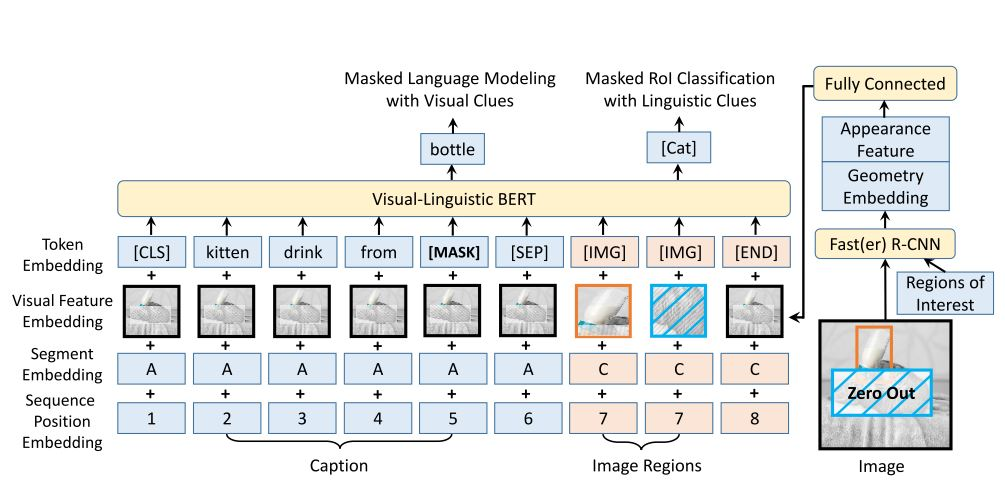
\includegraphics[scale=0.5]{images/VLBERT.JPG}}
		\caption[معماری شبکه از قبل آموزش‌دیده\lr{VL-BERT}]{معماری شبکه از قبل آموزش‌دیده\lr{VL-BERT}\cite{su2019vl}}
		\label{fig:VLBERT}
	\end{figure}

	شکل
	\ref{fig:VLBERT}
	معماری 
	\lr{VL-BERT}
		را نشان می‌دهد. مشابه 
	\lr{BERT}
	، از کدگذارهای
	\lr{multi-layer bidirectional transformer}
	استفاده شده است. اما برخلاف 
	\lr{BERT}
	که ورودی آن تنها کلمات جمله هستند، این شبکه به همراه کلمات یک جمله، مناطق مورد علاقه
	\footnote{\lr{regions-of-interest}}
	استخراج شده از تصویر و یا به اختصار
	\lr{ROI}
	را نیز به عنوان ورودی می‌گیرد. برای استخراج 
	\lr{ROI}
	از تصویر از شبکه 
	\lr{Faster RCNN}\cite{ren2015faster}
	استفاده شده است. هر ورودی این شبکه با توکن 
	\lr{[CLS]}
	آغاز می‌شود. سپس با کلمات جمله و 
	\lr{ROI}
	های تصویر ادامه می‌یابد و با توکن
	\lr{[END]}
	خاتمه می‌یابد. از توکن 
	\lr{[SEP]}
	نیز برای جدا کردن جملات و یا جملات و تصویر از هم استفاده می‌شود. برای هر ورودی، تعبیه ویژگی
	\footnote{\lr{feature embedding}}
	 آن جمع چهار نوع تعبیه است که در شکل 
	\ref{fig:VLBERT}
	 مشخص شده است. در میان آن‌ها، تعبیه مربوط به ویژگی‌های تصویری 
	\footnote{\lr{visual feature embedding}}
	 به تازگی به شبکه اضافه شده است در حالی که سه تعبیه دیگر از قبل در  مدل 
	\lr{BERT}
	 وجود داشته است. برای آموزش
	\lr{VL-BERT}
	از مجموعه‌ داده
	\lr{Conceptual Captions}
	به عنوان مجموعه‌داده زبانی- تصویری استفاده شده است. علاوه بر این از دو مجموعه‌داده فقط زبانی به نام‌های 
	\lr{BooksCorpus}
	و 
	\lr{English Wikipedia}
	به منظور بهبود تعمیم‌دهی شبکه استفاده شده است. برای بهینه‌سازی شبکه 
	\lr{VL-BERT}
	از دو تابع هدف استفاده شده است: 
	\lr{text-based Masked Language Model}
	و
	\lr{visual-based Masked Language Model}.
	در
	\lr{text-based Masked Language Model}
	با احتمال 15 درصد یکی از کلمات ورودی با توکن
	\lr{[MASK]}
	جایگزین می‌شود. بنابراین شبکه باید سعی کند که این کلمه ماسک شده را با توجه به کلمات دیگر و ویژگی‌های تصویری در خروجی پیش‌بینی نماید. در 
	\lr{visual-based Masked Language Model}
	با احتمال 15 درصد یکی از 
	\lr{ROI}
	ها ماسک ‌می‌شود و شبکه باید سعی کند در خروجی برچسب گروه مربوط به آن 
	\lr{ROI}
	را باتوجه به کلمات و سایر 
	\lr{ROI}
	ها پیش‌بینی کند. دقت شود که همانطور که در قسمت سمت راست تصویر
	\ref{fig:VLBERT}
	مشخص است، ملاک برچسب گروه‌بندی درست برای
	\lr{ROI}
	ها، خروجی شبکه
	\lr{Faster RCNN}
	است. 
	\begin{figure}
		\centerline{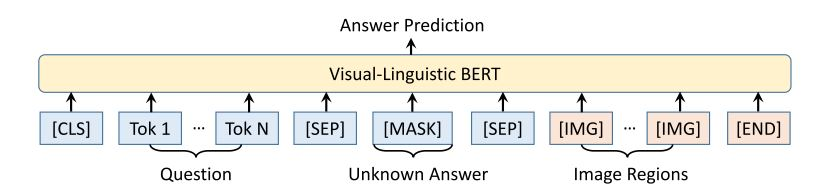
\includegraphics[scale=0.6]{images/VLBERT_finetuning.JPG}}
		\caption[نحوه ورودی و خروجی شبکه\lr{VL-BERT} برای آموزش در مسئله پرسش و پاسخ تصویری]{نحوه ورودی و خروجی شبکه\lr{VL-BERT} برای آموزش در مسئله پرسش و پاسخ تصویری\cite{su2019vl}}
		\label{fig:VLBERT-finetuning}
	\end{figure}
	برای استفاده از شبکه از قبل آموزش‌دیده
	\lr{VL-BERT}
	برای مسئله پرسش و پاسخ تصویری، مطابق شکل
	\ref{fig:VLBERT-finetuning}
	سه تایی کلمات سوال، پاسخ و 
	\lr{ROI}
	های استخراج‌شده از تصویر توسط
	\lr{Faster RCNN}
	در ورودی داده می‌شود که به جای پاسخ،
	\lr{[MASK]}
	قرار گرفته که شبکه تلاش می‌کند؛ پاسخ را در خروجی پیش‌بینی کند.
	
	\begin{figure}
		\centerline{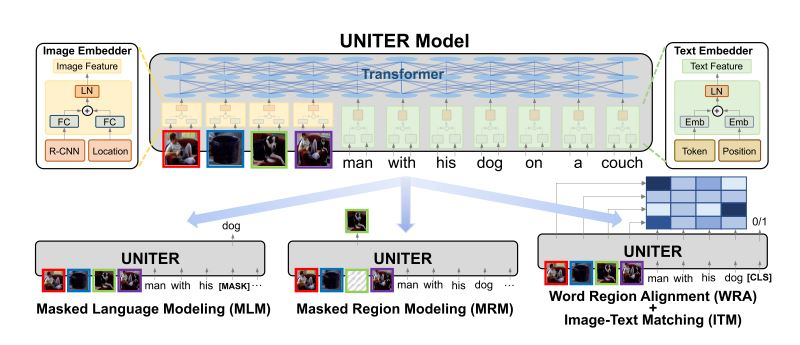
\includegraphics[scale=0.6]{images/UNITER.JPG}}
		\caption[معماری شبکه از قبل آموزش‌دیده\lr{UNITER}]{معماری شبکه از قبل آموزش‌دیده \lr{UNITER}\cite{chen2020uniter}}
		\label{fig:UNITER}
	\end{figure}
	معماری مدل 
	\lr{UNITER}
	در شکل
	\ref{fig:UNITER}
	نشان داده شده است. ورودی این مدل مانند
	\lr{VL-BERT}
	،کلمات یک جمله به همراه 
	\lr{ROI}
	های تصویر است. یکی از تفاوت‌های مدل 
	\lr{UNITER}
	با مدل 
	\lr{VL-BERT}
	این است که از 4 مجموعه‌داده زبانی-تصویری برای آموزش استفاده کرده است:(1)
	\lr{COCO}
	،(2)
	\lr{Visual Genome (VG)}
	،(3)
	\lr{Conceptual Captions}
	و(4)
	\lr{SBU Captions}.
	تفاوت دیگر این مدل با مدل
	\lr{VL-BERT}
	در توابع هدف است که علاوه بر
	\lr{text-based Masked Language Model}
	و
	\lr{visual-based Masked Language Model}
	از دو تابع هدف دیگر به نام‌های
	\lr{Image-Text Matching}
	و 
	\lr{Word-Region Alignment}
	نیز استفاده می‌کند. در
	\lr{Image-Text Matching}
	هدف این است که مدل بتواند پیش‌بینی کند که آیا جمله و تصویر داده شده در ورودی با هم مطابقت دارند یا خیر. بدین منظور، یک جمله و 
	\lr{ROI}
	های تصویر به 
	\lr{UNITER}
	داده می‌شود و در خروجی بازنمابی مربوط به توکن 
	\lr{[CLS]}
	از یک تابع سیگموئید عبور داده می‌شود که یک مقدار بین صفر و یک را برمی‌گرداند که مقدار یک نشان می‌دهد که جمله و تصویر ورودی کاملا با هم مطابقت دارد و مقدار صفر به این معناست که جمله و تصویر ورودی با هم مطابقت ندارد. در 
	\lr{UNITER}
	علاوه بر ‌در نظر گرفتن تطابق جمله و تصویر، از تطابق بین کلمات موجود در جمله و 
	\lr{ROI}
	های تصویر نیز برای آموزش استفاده می‌شود که این موضوع در قالب تابع هدف 
	\lr{Word-Region Alignment}
	در مدل مطرح شده است. زمان آموزش مدل 
	\lr{UNITER}
	به ازای هر دسته از داده‌های ورودی، یکی از 4 تابع هدف نامبرده شده به صورت تصادفی انتخاب می‌شود و براساس آن تابع هدف، عملیات کاهش گرادیان برای شبکه انجام ‌می‌شود. برای استفاده از شبکه از قبل آموزش‌دیده
	\lr{UNITER}
	برای مسئله پرسش و پاسخ تصویری، بازنمایی حاصل از توکن
	\lr{[CLS]}
	به یک شبکه 
	\lr{MLP}
	داده می‌شود و پاسخ را برای سوال و تصویر ورودی پیش‌بینی می‌کند. در واقع در این حالت، مسئله پرسش و پاسخ تصویری به عنوان یک مسئله طبقه‌بندی در نظر گرفته می‌شود.
	\begin{figure}
		\centerline{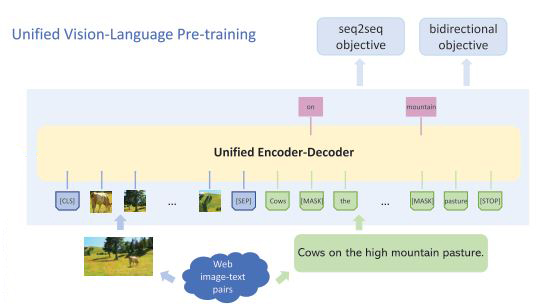
\includegraphics[scale=0.7]{images/VLP.JPG}}
		\caption[معماری شبکه از قبل آموزش‌دیده\lr{VLP}]{معماری شبکه از قبل آموزش‌دیده\lr{VLP}\cite{zhou2020unified}}
		\label{fig:VLP}
	\end{figure}
	
	شبکه از قبل آموزش‌دیده
	\lr{VLP}
	نیز مانند دو شبکه‌ی قبلی از کلمات یک جمله و
	\lr{ROI}
	های استخراج شده از تصویر به عنوان ورودی استفاده می‌کند. تفاوت اصلی این شبکه با دو شبکه
	\lr{VL-BERT}
	و 
	\lr{UNITER}
	در این است که یک شبکه‌ی یکپارچه رمزگذار-رمزگشا است که نه تنها در مسائل 
	\lr{understanding}
	بلکه در مسائل
	\lr{generative}
	به دلیل وجود رمزگشا قابل استفاده است. مدل 
	\lr{VLP}
	بر روی  مجموعه‌داده
	\lr{Conceptual Captions}
	آموزش داده شده است. دو تابع هدف در شبکه
	\lr{VLP} 
	استفاده شده است: (1) 
	\lr{bidirectional}
	و 
	\lr{seq2seq}.
	در تابع هدف
	\lr{bidirectional}
	یکی از کلمات موجود در جمله با توکن 
	\lr{[MASK]}
	جایگزین می‌شود و برای پیش‌بینی این کلمه ماسک شده در خروجی از تمامی کلمات و 
	\lr{ROI}
	های اطراف آن استفاده می‌شود. اما در تابع هدف 
	\lr{seq2seq}
	برای پیش‌بینی کلمه ماسک شده در خروجی، تنها از کلمات سمت چپ کلمه ماسک شده و 
	\lr{ROI}
	های اطراف آن استفاده می‌کند. به عبارتی دیگر، برای پیش‌بینی کلمه ماسک شده نمی‌توان از کلماتی که بعد از  آن و در آینده در جمله آمده است؛ استفاده کرد. معماری شبکه 
	\lr{VLP}
	در شکل 
	\ref{fig:VLP}
	نشان داده شده است.
	
	ورودی سه مدل قبلی یعنی 
	\lr{VL-BERT}
	،
	\lr{UNITER}
	و 
	\lr{VLP}
	یک جمله به همراه 
	\lr{ROI}
	های استخراج شده از تصویر بود. در مدل 
	\lr{OSCAR}
	علاوه بر این دو ورودی از ورودی دیگری به نام برچسب اشیا
	\footnote{\lr{object tag}}
	استفاده می‌شود که اشیایی که هم در تصویر وجود دارد و هم در جمله به آن اشاره شده است را نشان می‌دهد. در 
	\cite{li2020oscar}
ادعا شده است که استفاده برچسب اشیا منجر به تولید بازنمایی بهتری از متن و تصویر می‌شود و در واقع از این برچشب‌ها به عنوان لنگر برای تطابق دادن فضای تصویر و متن استفاده می‌شود. در مدل
	\lr{OSCAR}
	برای بدست آوردن 
	\lr{ROI}
	های تصویر و برچسب اشیا از شبکه 
	\lr{Faster RCNN}
	استفاده شده است. در مدل 
	\lr{OSCAR}
	به دو طریق می‌توان به ورود‌ی‌ها نگاه کرد که در نتیجه دو تابع هدف برای آموزش این شبکه تعریف می شود. در روش اول، کلمات جمله و برچسب اشیا با هم در نظر گرفته می‌شود (دید \lr{Dictionary}) و به احتمال 15 در صد یکی از کلمات جمله و یا یکی از برچسب‌های اشیا با توکن 
	\lr{[MASK]}
	جایگزین می‌شود و مدل باید سعی کند این کلمه ماسک شده را در خروجی پیش‌بینی کند
	(\lr{Masked Token Loss}).
	در روش دوم،
	\lr{ROI}
	های تصویر و برچسب اشیا با هم در نظر گرفته می‌شود(دید \lr{Modality}) و با احتمال 50 درصد برچسب‌های اشیا با برچسب‌های دیگری تغییر می‌کند و مدل باید پیش‌بینی کند که آیا کلمات موجود در جمله با قسمت برچسب اشیا و 
	\lr{ROI}
	های تصویر مطابقت دارد یا نه. که بدین منظور خروجی شبکه برای توکن
	\lr{[CLS]}
	به یک شبکه کاملا متصل داده می‌شود و یک طبقه‌بندی باینری انجام می‌شود که یک به معنای تطابق کلمات جمله با 
	\lr{ROI}
	های تصویر و برچسب اشیاست و صفر نشان‌دهنده عدم تطابق است(\lr{Contrastive Loss}).  برای آموزش مدل 
	\lr{OSCAR}
	از مجموعه‌داده‌های
	\lr{COCO}
	،
	\lr{Conceptual Captions}
	،
	\lr{SBU captions}
	،
	\lr{flicker30}
	و
	\lr{GQA}
	استفاده شده است. برای استفاده از شبکه از قبل آموزش‌دیده
	\lr{OSCAR}
	برای مسئله پرسش و پاسخ تصویری، سوال به همراه برچسب اشیا و 
	\lr{ROI}
	های تصویر به ورودی شبکه داده ‌می‌شود و خروجی توکن
	\lr{[CLS]}
	به یک طبقه‌بند داده ‌می‌شود تا پاسخ سوال و تصویر داده شده در تصویر بدست آید. در واقع در این روش، مسئله پرسش و پاسخ تصویری به صورت یک مسئله طبقه‌بندی در نظر گرفته ‌می‌شود.
	\begin{figure}
		\centerline{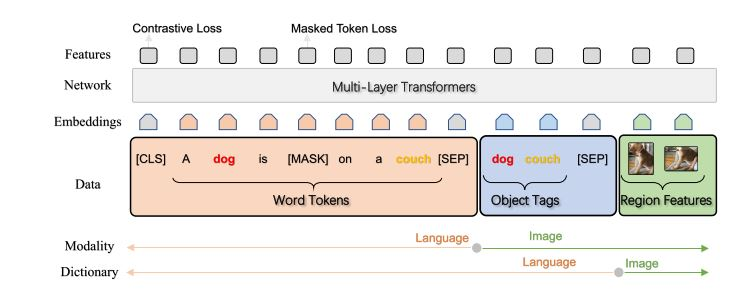
\includegraphics[scale=0.7]{images/OSCAR.JPG}}
		\caption[معماری شبکه از قبل آموزش‌دیده\lr{OSCAR}]{معماری شبکه از قبل آموزش‌دیده\lr{OSCAR}\cite{li2020oscar}}
		\label{fig:OSCAR}
	\end{figure}
	معماری شبکه 
	\lr{OSCAR}
	در شکل 
	\ref{fig:OSCAR}
	نمایش داده شده است.
	
\subsection[معماری دو جریان]{معماری دو جریان}
در مقابل معماری تک جریان، معماری‌ دو جریان برای یادگیری  هر کدام از بازنمایی‌های تصویر و متن از یک رمزگذار مستقل استفاده می‌کند. سپس از یک رمزگذار دیگر برای بدست آوردن بازنمایی مشترک متن و تصویر استفاده می‌کند.مشابه معماری تک جریان، معماری‌های دو جریان نیز مدل‌های خود را با
	\lr{visual-based Masked Language Model}
	،
	\lr{text-based Masked Language Model}
	و 
	\lr{visual-linguistic matching}
	بهینه می‌کنند. 
	\lr{ViLBERT}\cite{lu2019vilbert}
	 و
	\lr{LXMERT}\cite{tan2019lxmert}
  نمونه‌هایی از معماری دو جریان هستند که از این دو مدل می‌توان برای مسئله پرسش و پاسخ تصویری استفاده کرد. پس در ادامه این بخش، جزئیات این دو شبکه را بررسی خواهیم کرد.
  
	\begin{figure}
	 	\centerline{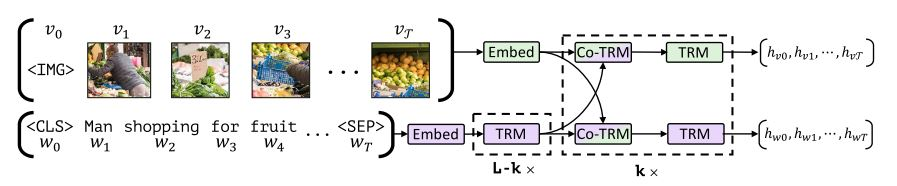
\includegraphics[scale=0.6]{images/VilBERT.JPG}}
	 	\caption[معماری شبکه از قبل آموزش‌دیده\lr{ViLBERT}]{معماری شبکه از قبل آموزش‌دیده\lr{ViLBERT}\cite{lu2019vilbert}}
	 	\label{fig:ViLBERT}
	\end{figure}
	
	شکل
	\ref{fig:ViLBERT}
	معماری شبکه 
	\lr{ViLBERT}
	را نمایش می‌دهد. مدل 
	\lr{ViLBERT}
	شامل دو مدل موازی به سبک
	\lr{BERT}
	است که به صورت جداگانه بر روی کلمات متن و 
	\lr{ROI}
	های تصویر اعمال می‌شود و از بلوک‌های ترنسفورمر در هر جریان استفاده شده است(در شکل 
	\ref{fig:ViLBERT}
	با 
	\lr{TRM}
	مشخص شده است.). سپس برای بدست آوردن بازنمایی مشترک بین متن و تصویر از لایه‌های 
	\lr{co-attentional transformer}
	استفاده شده است(در شکل 
	\ref{fig:ViLBERT}
	با 
	\lr{Co-TRM}
	مشخص شده است.). اساس لایه‌ی 
	\lr{co-attentional transformer}
    بر پایه‌ی ترنسفرمر است در واقع برای هر کدام از بخش‌های تصویری و متنی داده ورودی، یک ترنسفرمر در لایه 
    \lr{co-attentional transformer}
    در نظر گرفته شده است که پس از عبور متن و داده از جریان‌های مستقل خود و بدست آمدن 
	\lr{query}
	،
	\lr{key}
	و
	\lr{value}
	برای هر کدام، 
	\lr{key}
	و
	\lr{value}
	متن به ترنسفرمر تصویر در 
	\lr{co-attentional transformer}
	داده می‌شود و به صورت متقابل
	\lr{key}
	و
	\lr{value}
	تصویر به ترنسفرمر متن داده می‌شود. 
	
	\begin{figure}
		\centerline{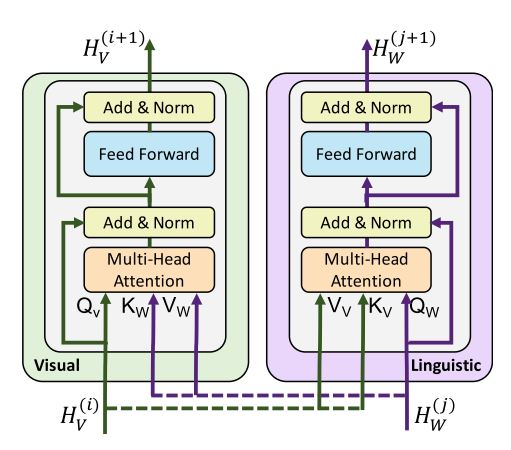
\includegraphics[scale=0.6]{images/coattentional.JPG}}
		\caption[ساختار لایه \lr{co-attentional transformer}]{ساختار لایه \lr{co-attentional transformer}\cite{lu2019vilbert}}
		\label{fig:coattentional}
	\end{figure}
	شکل 
	\ref{fig:coattentional}
	ساختار لایه
	\lr{co-attentional transformer}
	را نشان می‌دهد. برای آموزش مدل
	\lr{ViLBERT}
	از توابع هدف
	\lr{visual-based Masked Language Model}
	،
	\lr{text-based Masked Language Model}
	و 
	\lr{visual-linguistic matching}
	استفاده شده است. شبکه
	\lr{ViLBERT}
	بر روی مجموعه‌داده
	\lr{Conceptual Captions}
	آموزش داده شده است. برای استفاده از شبکه از قبل آموزش‌دیده
	\lr{ViLBERT}
	برای مسئله پرسش و پاسخ تصویری، ابتدا خروجی بازنمایی توکن
	\lr{[CLS]}
	و بازنمایی تصویر ضرب متناظر می‌شوند. سپس با عبور از یک شبکه 
	\lr{MLP}
	دولایه پاسخ مربوط به سوال و تصویر حاصل می‌شود.
	
	\begin{figure}
		\centerline{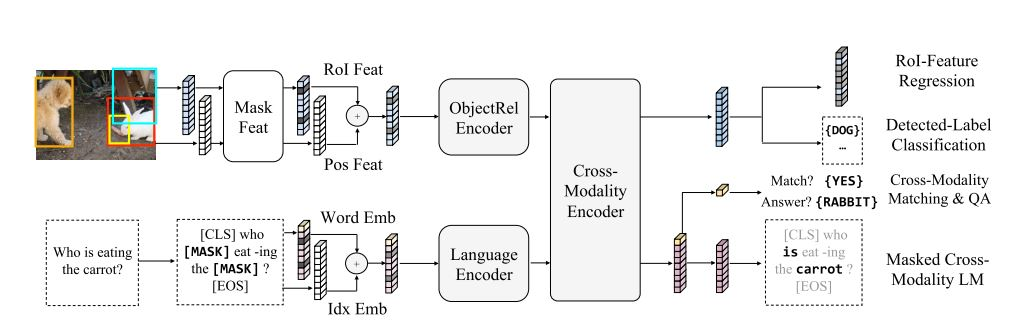
\includegraphics[scale=0.6]{images/LXMERT.JPG}}
		\caption[ معماری شبکه از قبل آموزش‌دیده \lr{LXMERT}]{معماری شبکه از قبل آموزش‌دیده \lr{LXMERT}\cite{tan2019lxmert}}
		\label{fig:LXMERT}
	\end{figure}
	
	شکل 
	\ref{fig:LXMERT}
	معماری مدل
	\lr{LXMERT}
	را نشان می‌دهد. ورودی این شبکه کلمات جمله ورودی و 
	\lr{ROI}
	های استخراج شده از تصویر است. همان‌طور که قبلا اشاره شد؛ مدل
	\lr{LXMERT}
	یک مدل دو جریان است به همین دلیل برای پردازش متن و تصویر از دو رمزگذار مجزا و مستقل استفاده شده است(در شکل 
	\ref{fig:LXMERT}
	به ترتیب با عنوان‌های  
	\lr{ObjectRel Encoder}
	و 
	\lr{Language Encoder}
	برای تصویر و متن مشخص شده است.
	) و سپس برای بدست آوردن بازنمایی مشترک از رمزگذار
	\lr{Cross-modality}
	استفاده شده است. توابع هدف استفاده شده در مدل
	\lr{LXMERT}
	مشابه شبکه 
	\lr{ViLBERT}
	است اما در 
	\lr{LXMERT}
	از تابع هدف دیگری به نام 
	\lr{image question answering}
	برای آموزش شبکه استفاده شده است. زیرا حدود $1/3$ داده‌ای که برای آموزش این شبکه استفاده شده است؛ یک سوال در مورد تصویر ورودی است. بنابراین با تعریف تابع هدف 
	\lr{image question answering}
	مدل سعی ‌می‌کند تا پاسخ این سوال را در خروجی پیش‌بینی کند. برای آموزش شبکه
	\lr{LXMERT}
	از مجموعه‌داده‌های 
	\lr{MS COCO}
	،
	\lr{Visual Genome}
	،
	\lr{VQA v2.0}
	،
	\lr{GQA balanced version}
	و
	\lr{VG-QA}
	استفاده شده است.
	\begin{table}
		\caption{مقایسه بین شبکه‌های از قبل آموزش‌دیده بر روی زبان طبیعی و تصویر }
		\label{tabel:6}
		\centering
		\setlength\extrarowheight{1pt}
		\begin{tabularx}{\textwidth}{|B|S|M|B|B|}
			\hline
			\textbf{روش} & \textbf{معماری} &  \textbf{ورودی} & \textbf{مجموعه‌داده‌های استفاده شده برای آموزش} & \textbf{توابع هدف}\\
			\hline \hline
			
			\textbf{\cite{su2019vl}\lr{VL-BERT}}& تک جریان & کلمات جمله + \lr{ROI}های تصویر &\lr{Conceptual Captions + BooksCorpus + English Wikipedia}&
			\lr{text-based MLM + visual-based MLM}\\
			\hline
			
			\textbf{\cite{chen2020uniter}\lr{UNITER}}& تک جریان & کلمات جمله + \lr{ROI}های تصویر & \lr{COCO + Visual Genome + Conceptual Captions + 
			SBU Captions} & \lr{text-based MLM + visual-based MLM + Image-Text Matching + Word-Region Alignment}\\
			\hline
			
			\textbf{\cite{zhou2020unified}\lr{VLP}}& تک جریان & کلمات جمله + \lr{ROI}های تصویر  & \lr{Conceptual Captions} & \lr{bidirectional + seq2seq}\\
			\hline
			
			\textbf{\cite{li2020oscar}\lr{OSCAR}}& تک جریان & کلمات جمله + \lr{ROI}های تصویر+ برچسب اشیا & \lr{COCO + Conceptual Captions + SBU captions + 
			flicker30 + GQA} & \lr{Masked Token Loss + Contrastive Loss}\\
			\hline \hline
			
			\textbf{\cite{lu2019vilbert}\lr{ViL-BERT}}& دو جریان & کلمات جمله + \lr{ROI}های تصویر & \lr{Conceptual Captions } & \lr{text-based MLM + visual-based MLM + Image-Text Matching}\\
			\hline
			
			\textbf{\cite{tan2019lxmert}\lr{LXMERT}}& دو جریان & کلمات جمله + \lr{ROI}های تصویر & \lr{MS COCO + Visual Genome + VQA v2.0 + GQA balanced version + 
			VG-QA} & \lr{text-based MLM + visual-based MLM + Image-Text Matching + 
			Image Question Answering }\\
			\hline		
		\end{tabularx}
	\end{table}

	در جدول 
	\ref{tabel:6}
	مقایسه چند نمونه از مدل‌های از قبل آموزش‌دیده بر روی زبان طبیعی و تصویر که مسئله پرسش و پاسخ تصویری را پشتیبانی می‌کنند؛ آورده شده است. ورودی تمام این مدل‌ها،
	کلمات جمله و
	\lr{ROI}
	های تصویر است به جز مدل 
	\lr{OSCAR}
	که علاوه بر این دو، برچسب اشیا را نیز به عنوان ورودی دریافت می‌کند. شباهت دیگر این مدل‌ها در استفاده از مجموعه‌داده 
	\lr{Conceptual Captions}
	برای آموزش است البته به جز مدل 
	\lr{LXMERT}
	که از این مجموعه‌داده استفاده نکرده است. نکته‌ی حائز اهمیت دیگر در این جدول استفاده تقریباً تمامی مدل‌ها از دو تابع هدف
	\lr{text-based Masked Language Model}
	و
	\lr{visual-based Masked Language Model}
	است.
	
	\begin{table}
		\caption{دقت شبکه‌های از قبل آموزش‌دیده بر روی مجموعه‌داده 
		\lr{VQA v2.0 (test-std)}}
		\label{tabel:7}
		\begin{center}
			{\begin{tabular}{ |c|c|c|c|c| } 
					\hline
					\textbf{دقت کل} & \textbf{سایر سوالات} &  \textbf{سوالات شمارشی} & \textbf{سوالات بله/خیر} & \textbf{روش}\\
					\hline \hline	
					$70.7$  & $60.5$ & $52.1$ & $87.4$ &\textbf{\cite{zhou2020unified}\lr{VLP}} \\
					\hline
					$70.92$ & - & - & - &\textbf{\cite{lu2019vilbert}\lr{ViL-BERT}}\\
					\hline
					$72.22$ & - & - & - &\textbf{\cite{su2019vl}\lr{VL-BERT}}  \\
					\hline
					$72.5 $  & $63.1$ & $54.2$ & $88.2$ &\textbf{\cite{tan2019lxmert}\lr{LXMERT}}\\
					\hline
					$73.82$& - & - & - &\textbf{\cite{li2020oscar}\lr{OSCAR}}\\
					\hline
					$74.02$ & - & - & - &\textbf{\cite{chen2020uniter}\lr{UNITER}} \\
					\hline
			\end{tabular}}
		\end{center}
	\end{table}

	در جدول 
	\ref{tabel:7}
	نتایج مدل‌‌های 
	\lr{VL-BERT}
	،
	\lr{UNITER}
	،
	\lr{VLP}
	،
	\lr{OSCAR}
	،
	\lr{ViL-BERT}
	و
	\lr{LXMERT}
	بر روی مجموعه‌داده
	\lr{VQA v2.0}
	نشان داده شده است. بهترین نتیجه بدست آمده برای مدل
	\lr{UNITER}
	است. یکی از نکات قابل ملاحظه در این جدول این است که مدل‌های تک جریان نتایج بهتری نسبت به مدل‌های دو جریان بدست آوردند در حالی که تعداد پارامترهای مدل‌های تک جریان نسبت به مدل‌های دو جریان کمتر است.
	
	
	
	
	

\section{معیارهای ارزیابی مسئله پرسش و پاسخ تصویری}

در این بخش می‌خواهیم به طور مختصر معیارهای ارزیابی شناخته شده در مسئله پرسش و پاسخ تصویری را بررسی‌کنیم. همان‌طور که قبلا ذکر شد؛ معمولا دو نوع سوال در مجموعه‌داده‌های پرسش و پاسخ تصویری در نظر گرفته می‌شود: سوالات 
\lr{open-ended}
و سوالات چندگزینه‌ای. در سوالات چندگزینه‌ای، برای هر سوال دقیقا یک پاسخ صحیح وجود دارد. بنابراین ارزیابی آن ساده است زیرا می‌توان به راحتی از معیار دقت استفاده کرد. اما در سوالات
\lr{open-ended}
این امکان وجود دارد که چندین پاسخ صحیح برای هر سوال وجود داشته باشد. بنابراین ارزیابی در این حالت ساده نخواهد بود. برای حل این موضوع، اکثر مجموعه‌داده‌های پرسش و پاسخ تصویری پاسخ‌ها را محدود به چند کلمه(1 تا3 کلمه) می‌کنند و یا پاسخ‌ها را از یک مجموعه بسته انتخاب می‌کنند.

 در ادامه به بررسی  مهم‌ترین معیارهای این حوزه می‌پردازیم. اما ارزیابی مسئله پرسش و پاسخ تصویری همچنان یک مسئله حل نشده است. هر کدام از روش‌ها و معیارهای ارزیابی موجود، مزیت‌ها و معایب خاص خود را دارند. بنابراین برای انتخاب معیار ارزیابی باید به مواردی همچون ساختار مجموعه‌داده و نحوه‌ی ساخت آن، میزان بایاس موجود در مجموعه‌داده و ... توجه نمود. 

\subsection{معیار دقت}

		اگر چه در سوالات چندگزینه‌ای برای سنجش یک مدل معیار دقت کافی است اما در سوالات 
		\lr{open-ended}
		معیار دقت سخت‌گیرانه است زیرا فقط در حالتی که پاسخ مدل کاملا مطابق با پاسخ در نظر گرفته شده باشد، پذیرفته می‌‌شود. برای مثال اگر صورت سوال «چه حیواناتی در تصویر است؟» باشد و پاسخ مدل به جای «سگ‌ها‌» پاسخ «سگ» باشد؛ غلط تلقی می‌شود. بنابراین به دلیل این محدودیت‌هایی که معیار دقت دارد؛ معیارهای دیگری برای ارزیابی این نوع سوالات پیشنهاد‌ شده‌است.
		\begin{equation}
		Accuracy = \frac{Number \ of \ questions \ answered \ correctly}{Total \ questions}
		\end{equation}

	
\subsection[معیار شباهت \lr{Wu-Palmer}]{معیار شباهت \lr{Wu-Palmer}\cite{wu1994verb}}
	این معیار ارزیابی توسط مالینوفسکی 
	\cite{malinowski2014multi}
	برای پرسش و پاسخ تصویری ارائه شد. این معیار از تئوری مجموعه‌های فازی الهام گرفته شده است و نسبت به معیار دقت سخت‌گیری کمتری دارد. معیار شباهت 
	\lr{Wu-Palmer}
	سعی می‌کند که تفاوت بین پاسخ پیش‌بینی شده با پاسخ صحیح  را از لحاظ معنایی اندازه‌گیری‌کند. یکی از معایب این معیار این است که به پاسخ‌هایی که از لحاظ لغوی شبیه هم هستند ولی از لحاظ معنایی متفاوت هستند، امتیاز بالایی می‌دهد. زمانی که پاسخ‌های ما به صورت عبارت یا جمله باشد؛ این  معیار عملکرد خوبی ندارد. 

\subsection{معیار اجماع}

		از این معیار زمانی استفاده می‌شود که هر سوال توسط کاربرهای انسانی متفاوتی پاسخ داده شود. در واقع برای هر سوال چندین پاسخ مستقل وجود داشته باشد. این معیار دو نوع دارد: میانگین اجماع و کمترین اجماع. در میانگین اجماع امتیاز نهایی برابر با میانگین وزندار پاسخ‌های وارد شده توسط کاربرهای متفاوت است و در کمترین اجماع پاسخ پیش‌بینی شده حداقل باید با یکی از پاسخ‌ها مطابقت داشته باشد. در مسئله‌ی پرسش و پاسخ تصویری معمولا از حالت کمترین اجماع استفاده می‌شود و آستانه را هم برابر 3 قرار می‌دهند به این معنی که اگر پاسخ پیش‌بینی شده با 3 و یا بیشتر از 3 پاسخ برابر باشد امتیاز کامل می‌گیرد و در غیر این صورت هیچ امتیازی کسب نخواهد کرد. از معایب این روش می‌توان به هزینه زیاد جمع‌آوری پاسخ برای سوالات اشاره کرد. آنتول و همکارانش از این معیار ارزیابی در 
		\cite{antol2015vqa}
		استفاده کرده‌اند.
		\begin{equation}
			Accuracy_{VQA} = min(\frac{n}{3}, 1)
		\end{equation}

\subsection[\lr{MPT}]{\lr{MPT}\cite{kafle2017analysis}}

		یکی از مشکلات مجموعه‌داده‌های پرسش و پاسخ تصویری توزیع غیریکنواخت انواع سوال‌هاست. دراین مواقع، نمی‌توان از معیار دقت استفاده کرد. بنابراین  در 
	\cite{kafle2017analysis}
		 معیار جدیدی به نام 
	\lr{MPT} 
	\footnote{\lr{Mean Per Type}}
		ارائه شده است که توزیع نامتوازن سوال‌ها را جبران می‌کند. معیار 
	\lr{MPT}
	میانگین دقت برای هر نوع سوال را محاسبه می‌کند. از نسخه‌ی نرمالایز شده‌ی این معیار نیز برای رفع مشکل بایاس در توزیع پاسخ‌ها استفاده می‌شود.


\subsection[\lr{BLEU}]{\lr{BLEU}\cite{papineni2002bleu}}

		\lr{BLEU}
		\footnote{\lr{BiLingual Evaluation Understudy}}
		یکی از معیارهای ارزیابی خودکار ترجمه ماشینی است. در
		\cite{gurari2018vizwiz}
		 پیشنهاد داده شد که از این معیار نیز برای ارزیابی پرسش و پاسخ تصویری می‌توان استفاده کرد. معیار 
		\lr{BLEU}
		کنار هم قرار گرفتن 
		\lr{n-gram}
		های پاسخ پیش‌‌بینی شده و پاسخ صحیح را اندازه‌گیری می‌کند. معمولا
	\lr{BLEU}
	زمانی که جمله‌ها کوتاه باشند، با شکست مواجه می‌‌شود.
		


\subsection[\lr{METEOR}]{\lr{METEOR}\cite{denkowski2014meteor}}
		\lr{METEOR}
		\footnote{\lr{Metric for Evaluation of Translation with Explicit ORdering}}
		نیز همانند
		\lr{BLEU}
	یکی از معیارهای ارزیابی خودکار ترجمه ماشینی است. به پیشنهاد 
	\cite{gurari2018vizwiz}
	 از این معیار هم می‌توان برای پرسش و پاسخ تصویری نیز استفاده نمود. معیار 
		\lr{METEOR}
		سعی می‌کند که هم‌ترازی بین کلمات موجود در پاسخ پیش‌بینی شده و پاسخ صحیح را پیدا کند.
